% !TeX root = ../thuthesis-example.tex

\chapter{遗忘方法的实现与验证}

\section{实验验证}

\subsection{实验环境介绍}
我们用到的实验设备是两台服务器。
\begin{table}
    \centering
    \caption{实验设备情况}
    \begin{tabular}{lll}
      \toprule
      属性  & 设备1 & 设备2  \\
      \midrule
      CPU   & Core(TM) i9-9900K CPU @ 3.60GHz & Core(TM) i7-6700K CPU @ 4.00GHz \\
      内存大小  & 32G & 32G                    \\
      硬盘类型 & SSD  & SSD  \\
      显卡类型 & Nvidia Geforce 2080  & Nvidia Geforce 1080  \\
      显卡数量 & 1  & 3  \\
      操作系统 & ubuntu16.04LTS  & ubuntu16.04LTS  \\
      \bottomrule
    \end{tabular}
    \label{tab:model-attack-difference}
\end{table}

我们使用的深度学习框架Pytorch,数据集是CIFAR-10\cite{cifar10_2009},正常训练集50000张图片,测试集10000张图片。
遗忘两个类别,遗忘集是从正常训练集分离出来的10000张图片,遗忘测试集2000张图片。保留训练集是指正常训练集出去了遗忘集外的数据集合。
保留训练集40000张图片,保留测试集8000张图片。神经网络框架是Resnet18\cite{He_2016_CVPR}。

在训练时我们使用了自适应学习率的方法,自适应的策略是如果测试集平均损失函数连续3次低于历史最好值,则学习率减半。每次训练数量是100,初始学习率为0.1。随机梯度下降训练方法,权重衰减参数0.0005,冲量参数0.9。

\subsection{实验设计}
\subsubsection{确定冻结层数实验}
\begin{figure}
    \centering
    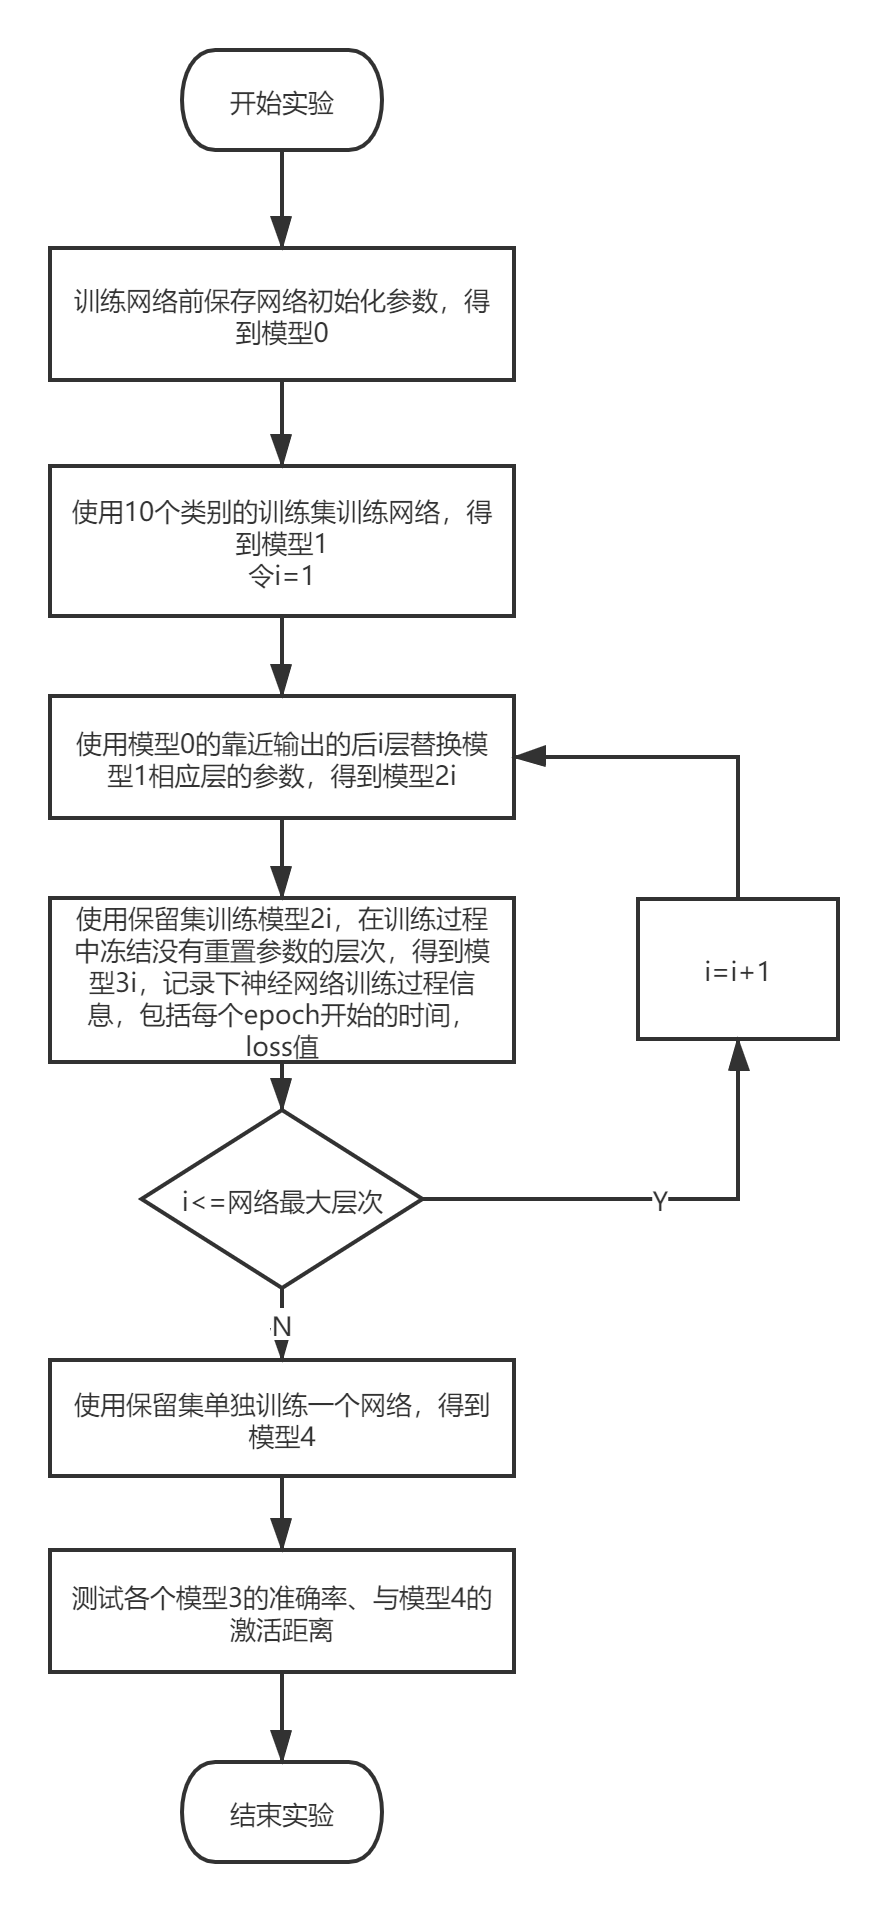
\includegraphics[scale=0.25]{chapter4_process_1.png}
    \caption{确定冻结层数实验流程图}
    \label{fig:chapter4_process_1}
\end{figure}

这个实验的目的是确定网络冻结的层次数。确定的标准是根据\ref{forget_evaluation_index}中讲到的三个指标的综合指标。
我们首先使用正常训练集去训练神经网络,直至训练集准确率收敛,获得模型1,在训练网络之前保存神经网络训练之前的网络参数,记为模型0。
将模型1的最后一层(全联接层)的参数替换为模型0的最后一层参数,模型1其余层数的参数不变,由此得到模型2\_1。
将模型2\_1加载到一个新的神经网络中,使用保留集去训练这个新的网络,直至训练准确率收敛,在训练过程中保持除全连接层以外层次的参数不被更新(即冻结),得到模型3\_1。
然后再将模型1的后两层参数替换为模型0的后两层参数,得到模型2\_2。将模型2\_2用保留集去训练至模型收敛,训练过程中保持未被更新的参数冻结,模型收敛后得到模型3\_2。
以此类推,逐层重置参数并且冻结参数使用保留集训练至模型收敛。
最后再使用保留集重新训练一个神经网络,获得模型4。
将每个模型3测量准确率、收敛时间和与模型4的激活距离,根据实验结果综合分析确定冻结层数。

\subsubsection{冻结必要性验证实验}
\begin{figure}
    \centering
    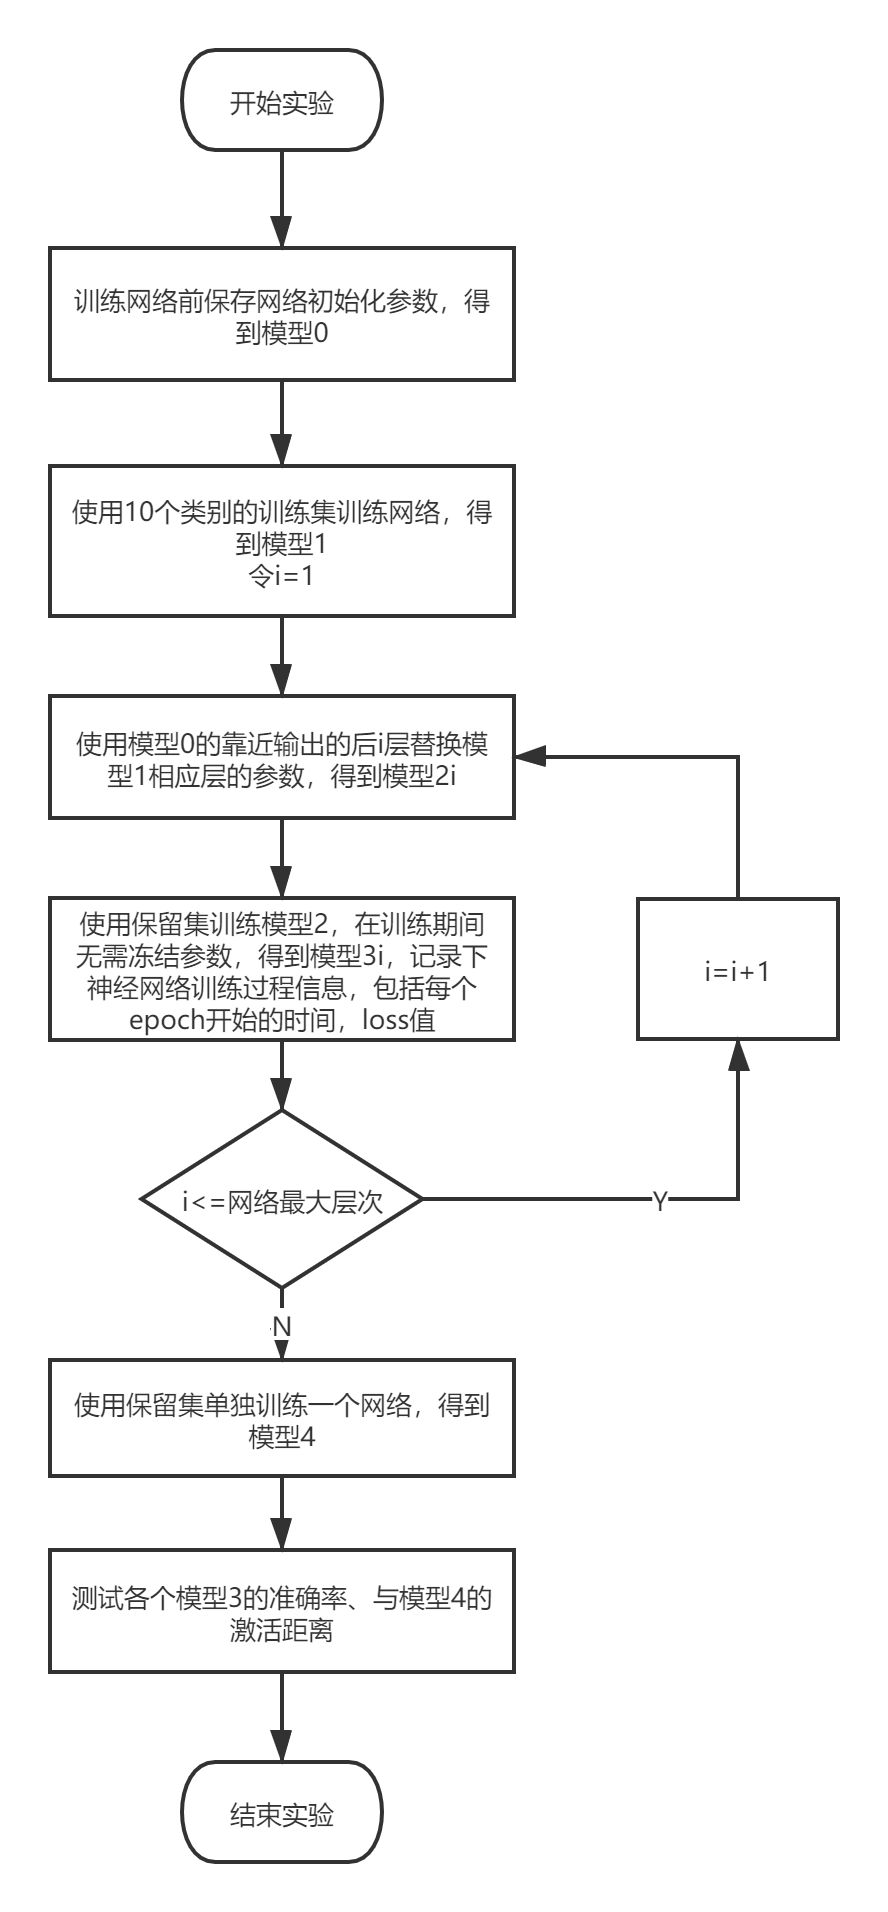
\includegraphics[scale=0.25]{chapter4_process_2.png}
    \caption{冻结必要性实验流程图}
    \label{fig:chapter4_process_2}
\end{figure}

通过本实验验证冻结较低层次的参数是否对加快遗忘训练收敛速度有一定的贡献,同时观察准确率以及激活距离的变化情况。
本实验的实验过程和确定冻结层数实验大致相同。不同的地方在于训练模型至收敛的过程中无需冻结参数,以对比冻结参数对遗忘效果的影响程度。
\subsubsection{反向冻结验证实验}
\begin{figure}
    \centering
    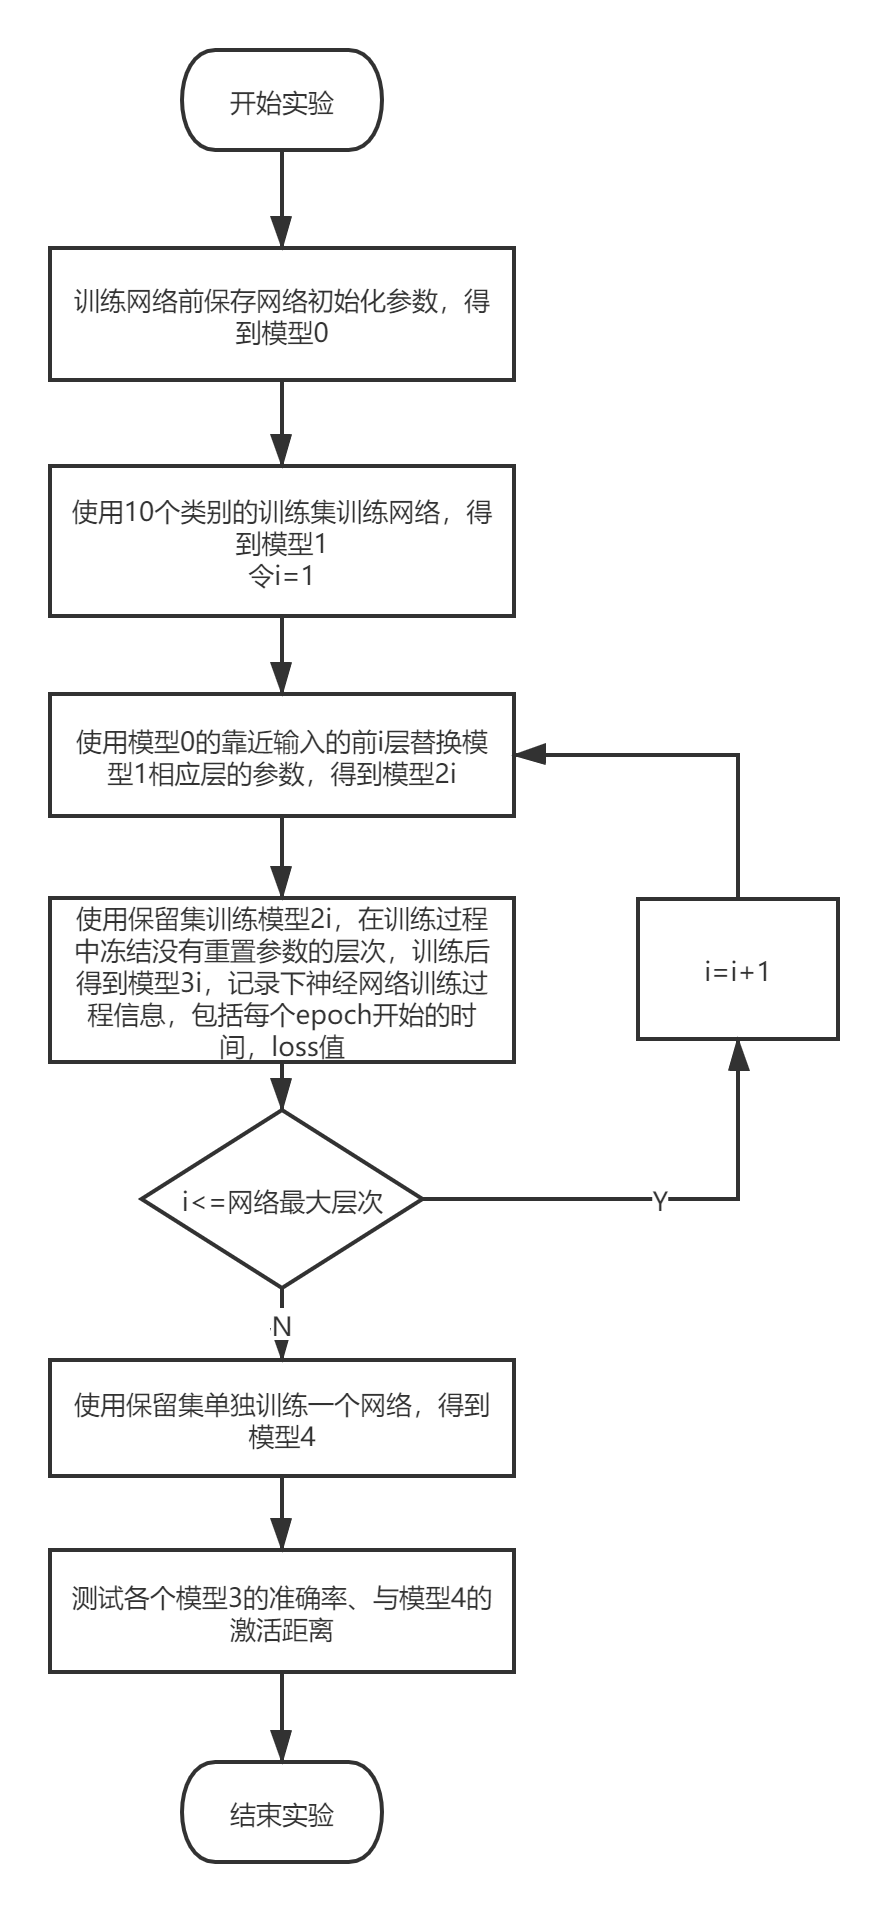
\includegraphics[scale=0.25]{chapter4_process_3.png}
    \caption{反向冻结验证实验流程图}
    \label{fig:chapter4_process_3}
\end{figure}

本实验是为了验证卷积神经网络的分层抽象特性,与正向冻结实验进行对照。
用正常训练集训练神经网络得到模型1,在正常训练集训练之前保留网络参数得到模型0。
用模型0的第一卷积层参数,替换模型1的第一卷积层参数,得到模型2\_1。
用神经网络加载模型2\_1,除了第一卷积层外,其余层数的参数全部冻结。用保留集训练至训练准确率收敛,得到模型3\_1。
然后再将模型0的第一层和第二层卷积参数替换模型1的相应层数的参数,得到模型2\_2。将模型2\_2除了前两层以外的全部参数冻结,使用保留集训练至模型收敛,得到模型3\_2。
以此类推,分别重置第一卷积层至最后一层全连接层参数,重复上述步骤。在实验过程中记录下每个epoch开始时间以及损失函数loss值。

\subsubsection{遗忘可持续性验证实验}
\begin{figure}
    \centering
    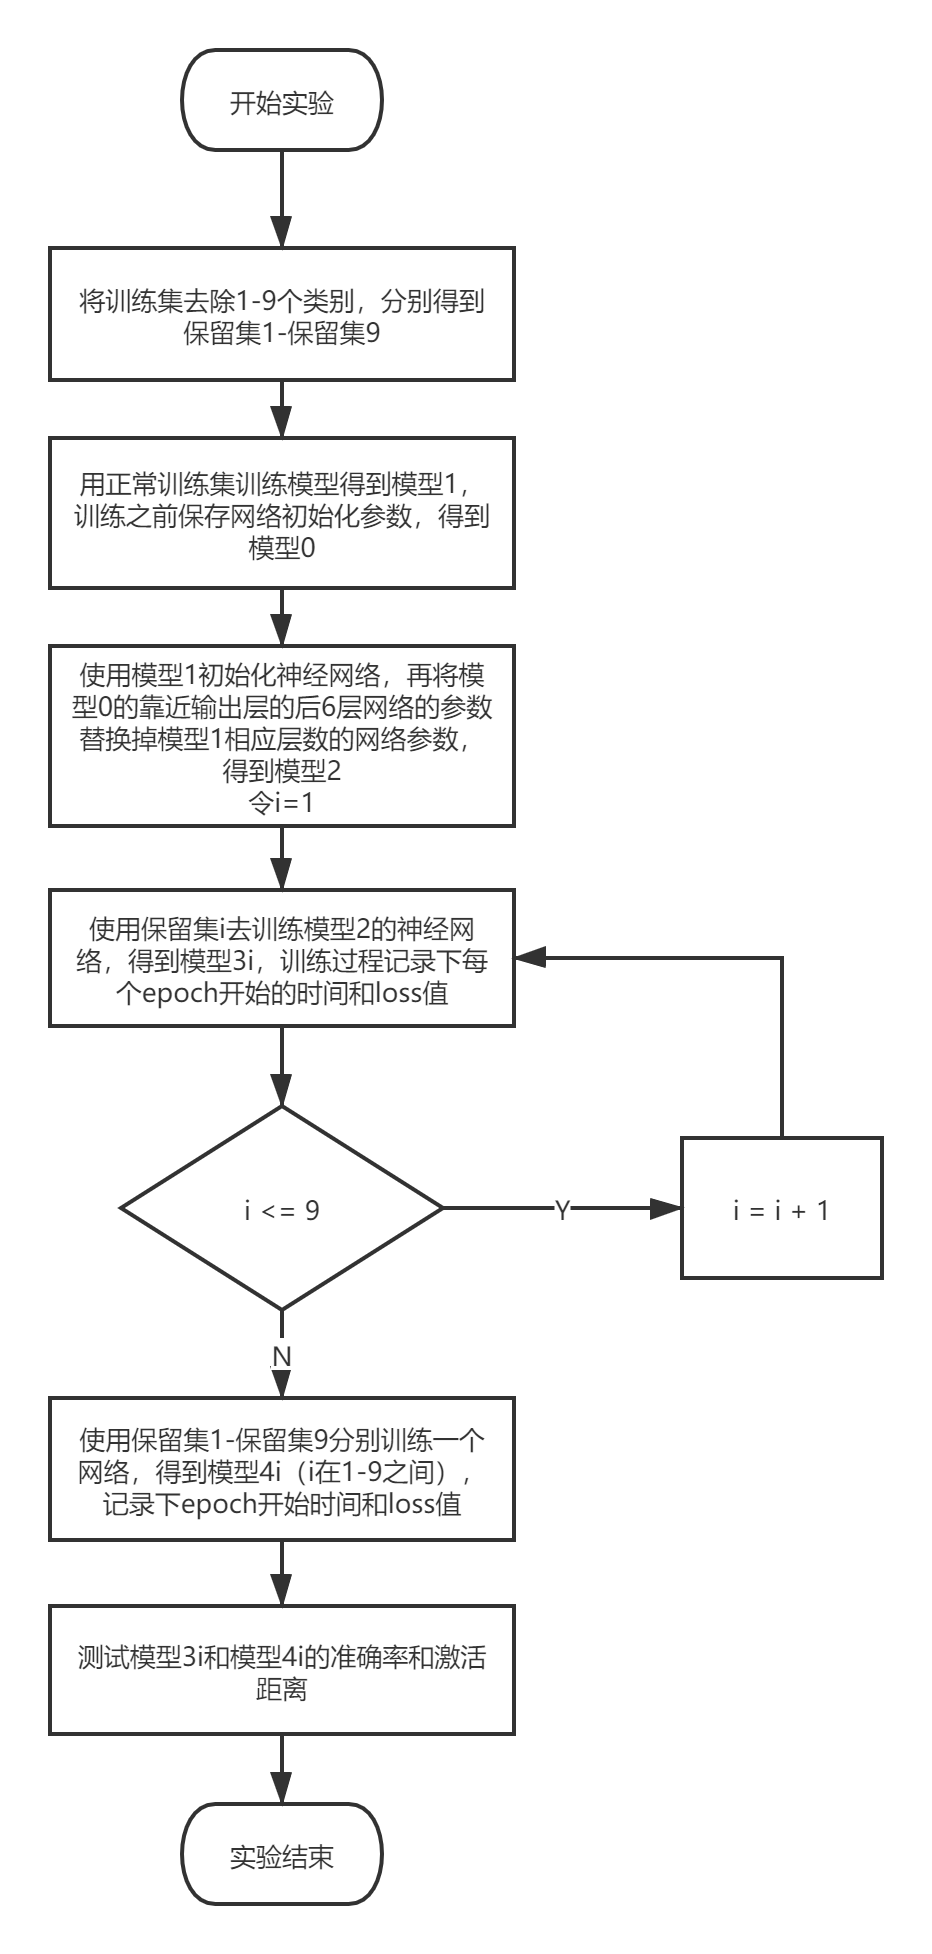
\includegraphics[scale=0.25]{chapter4_process_4.png}
    \caption{遗忘可持续性验证实验流程图}
    \label{fig:chapter4_process_4}
\end{figure}

本实验为了检验冻结重置方法随着遗忘类别数量的增多有效性的变化情况。
首先,将训练数据去除一个类别的数据,得到了保留集1,去掉两个类别的数据便得到了保留集2。以此类推,一共得到9个保留集。
用正常训练集训练神经网络得到模型1,在正常训练集训练之前保留网络参数得到模型0。
用神经网络加载模型1,然后把神经网络全连接层和靠近输出层的5层卷积层的参数重置为模型0的相应层次的参数,得到模型2\_1到模型2\_9。
然后分别用保留集1-保留集9去训练模型,训练过程中冻结除了全连接层和后6层卷积层的参数。得到模型3\_1到模型3\_9。
然后使用保留集1-保留集9分别重新训练模型,得到模型4\_1到模型4\_9。
训练过程中记录各epoch开始时间和损失函数loss值。
分别测试模型3\_1到模型3\_9,还有模型4\_1到模型4\_9的准确率、收敛时间以及激活距离。

\section{实验结果}
\subsection{确定冻结层数实验}
\begin{figure}
    \centering
    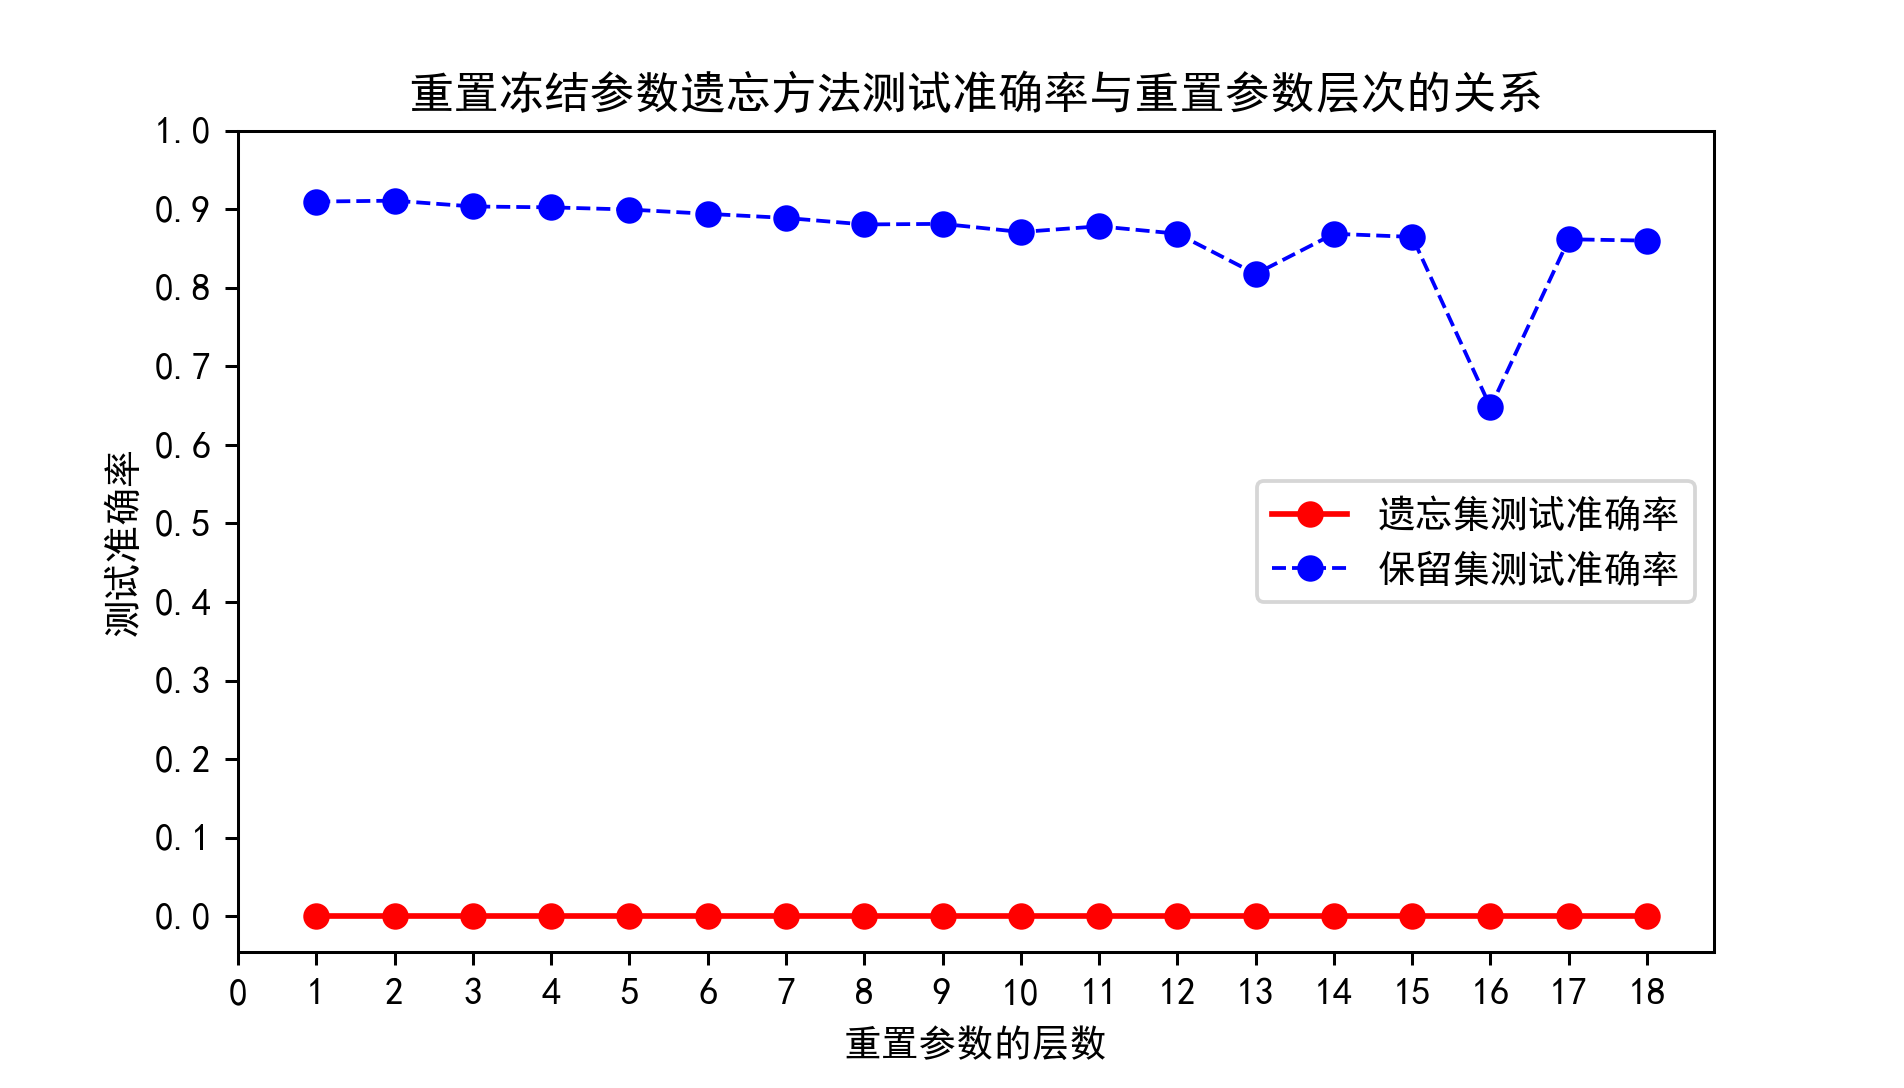
\includegraphics[width=0.9\linewidth]{chapter4_1.png}
    \caption{重置冻结参数遗忘方法测试准确率与重置参数层次的关系}
    \label{fig:chapter4_1}
\end{figure}

如图\ref{fig:chapter4_1}所示,图中展示了本文所讲述的重置冻结参数遗忘方法训练的网络用遗忘集和保留集训练之后得到测试准确率。
蓝色的折线代表利用保留测试集测试的准确率,红色的折线代表使用遗忘测试集测试的准确率的情况。
从红线可以看出,遗忘测试集的准确率全是0。这样的结果与完全重新训练得到的模型在遗忘测试集上的准确率完全相同。这说明使用本文提出的冻结重置参数方法,无论重置多少层参数,在遗忘集上均能达到理想的效果。
从蓝线与上面的点线可以看出,本方法得到的模型在保留集测试准确率上在大部分情况下均好于完全重新训练得到的模型在保留集上的准确率。
从蓝色圆点曲线中也发现随着重置参数的层数的增加,其保留集测试准确率有下降趋势,逐渐接近完全重新训练模型在保留集上的测试结果。
仅通过这一个方面还不足以让我们选出要重置参数的层次。
\begin{figure}
    \centering
    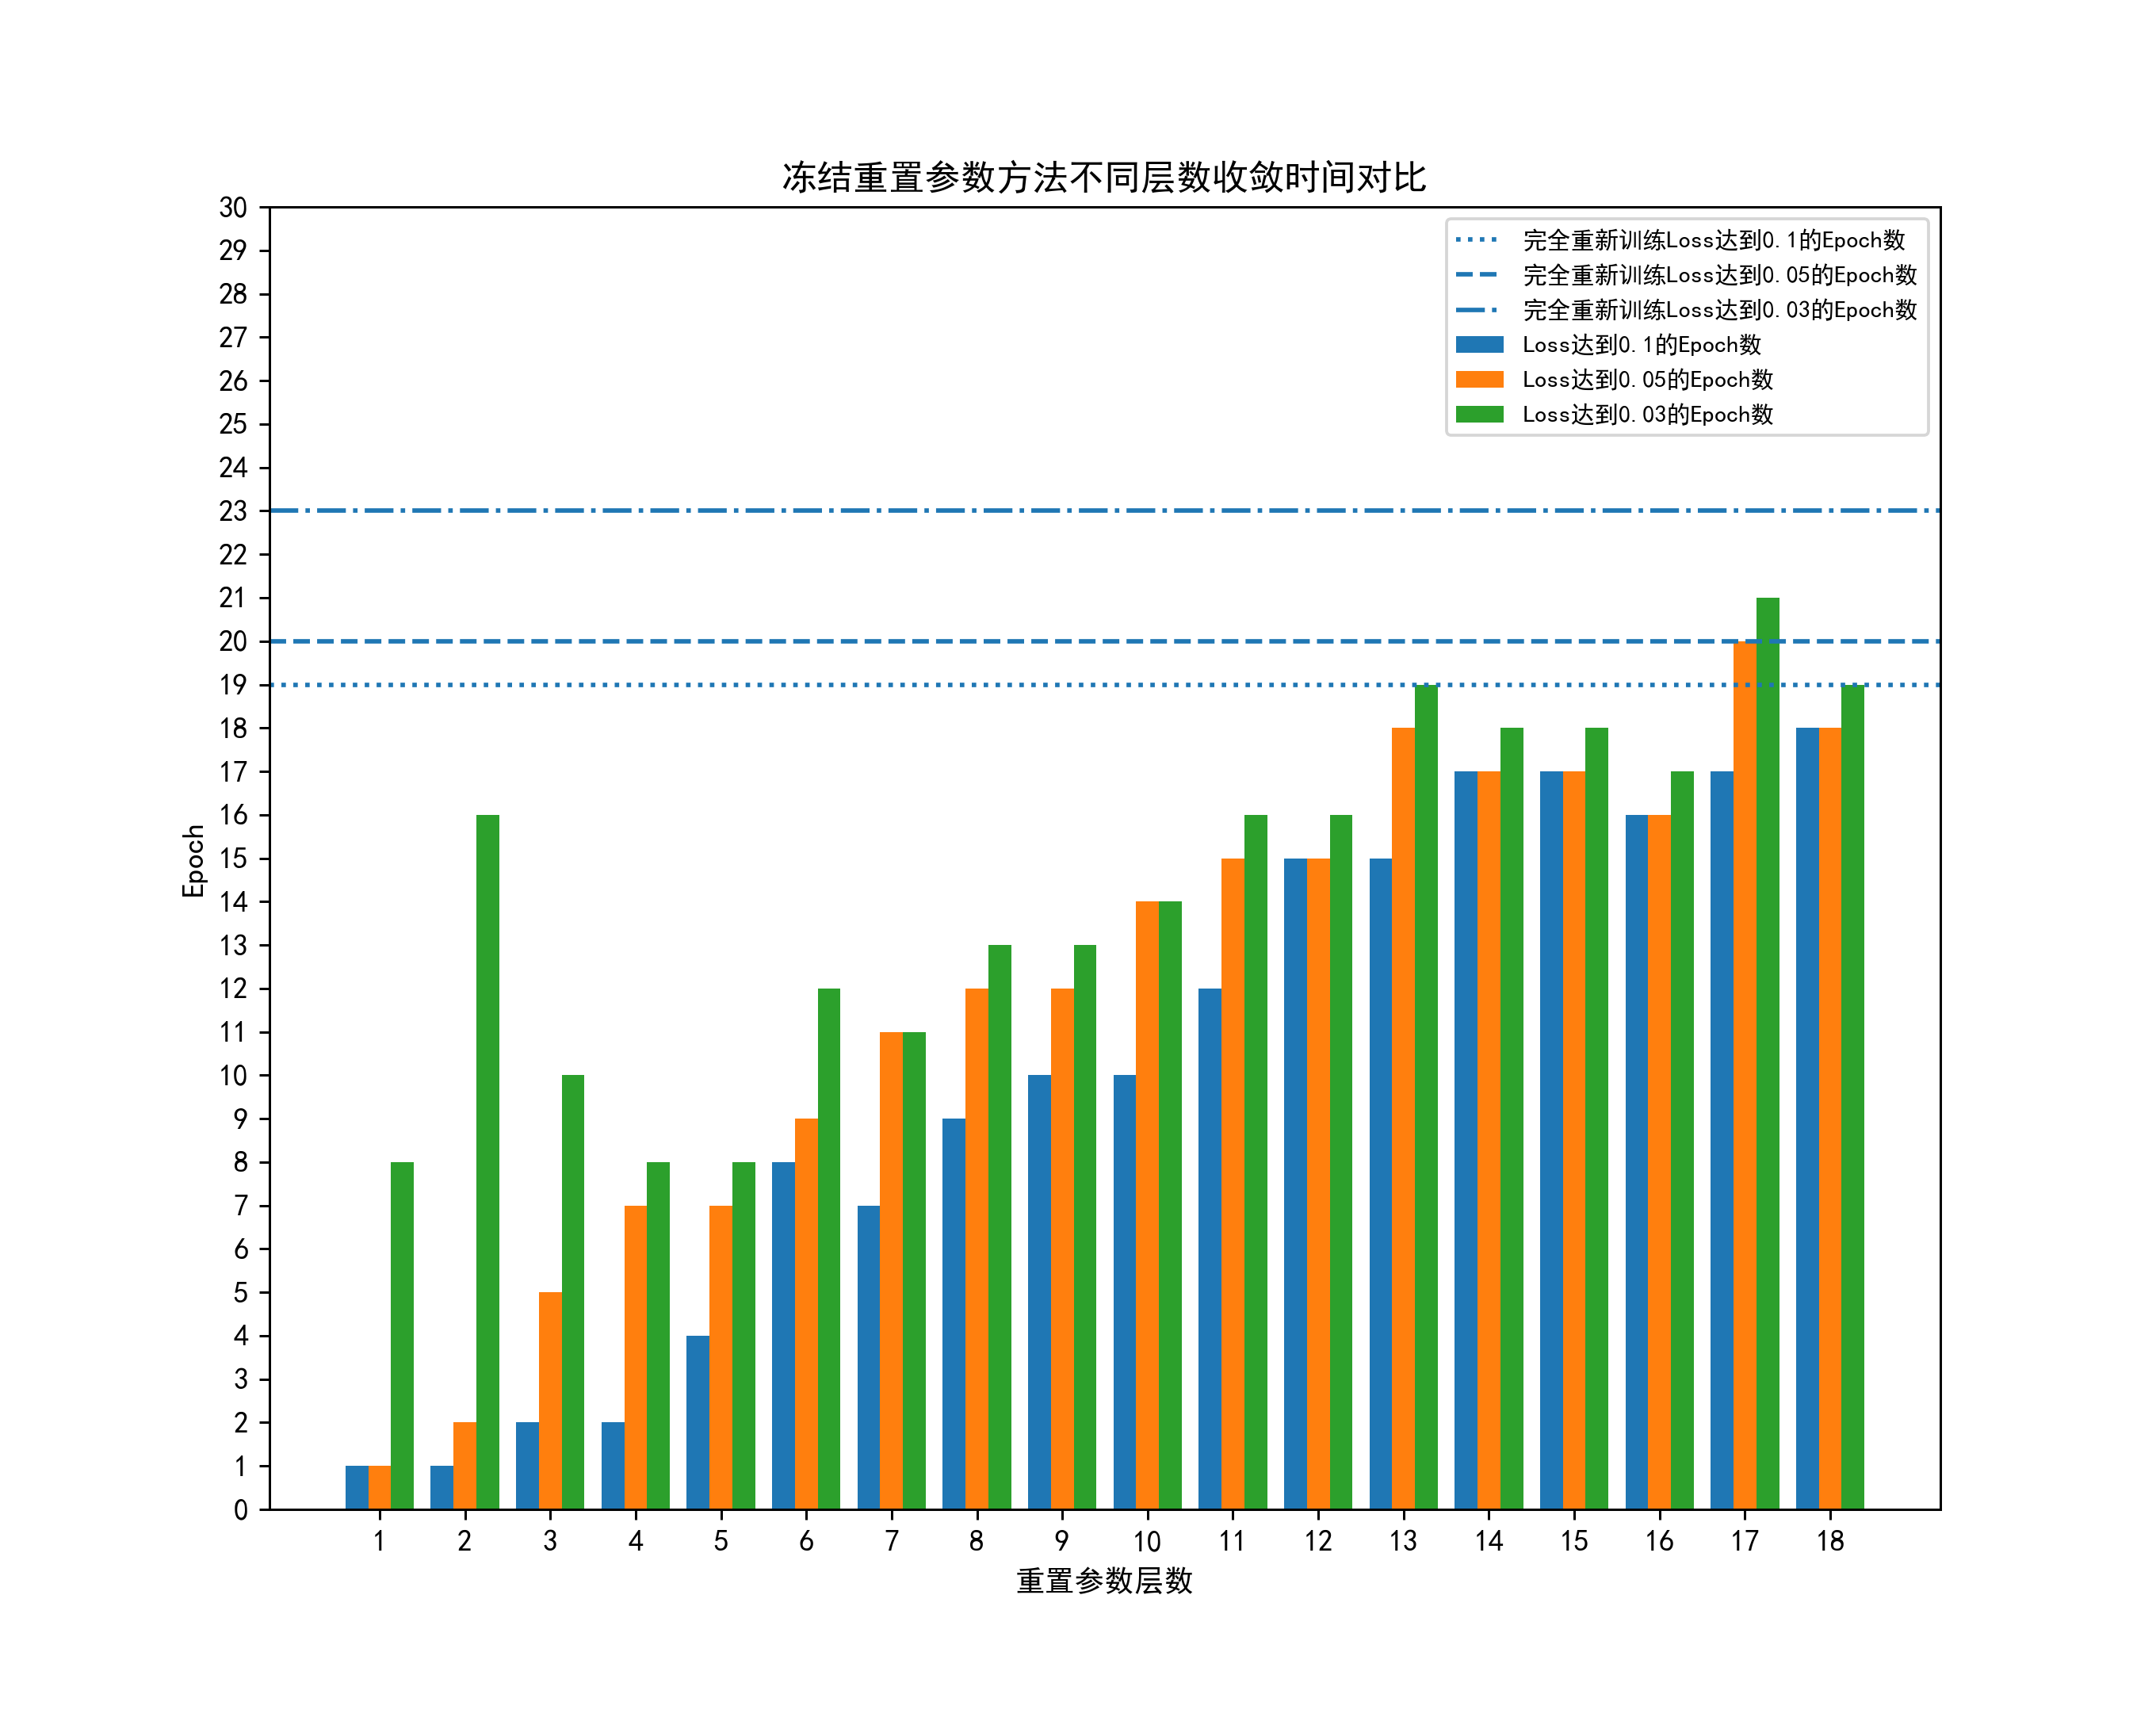
\includegraphics[width=1\linewidth]{chapter4_time_1.png}
    \caption{冻结重置参数方法不同层数收敛时间对比}
    \label{fig:chapter4_time_1}
\end{figure}

如图\ref{fig:chapter4_time_1}所示,图中展示了本文所讲述的重置冻结参数遗忘方法在重置不同层次参数上使用保留集训练后收敛时间的对比。
图中展示了三套柱状对比图,蓝色柱图、黄色柱图和绿色柱图分别代表使用保留训练集训练网络时,该训练批次(Epoch)的平均损失函数loss的值首次降到0.1,0.05和0.03以下时的训练批次(Epoch)数。
批次数越小,说明训练的收敛时间越快。上面有三条不同线型的横线,分别代表为了遗忘一定的类别完全重新训练网络,该训练过程的平均损失函数值首次降到0.1,0.05和0.03以下时的训练批次(Epoch)数。
这三条横线的作用时与本文提到的方法进行收敛时间上的对比。
从图中的柱状图中可以看出,随着重置参数的层数逐渐增多,其收敛的Epoch逐渐增大,逐渐接近完全重新训练时收敛的Epoch。
其实这也不难理解,随着重置参数的层数增多,网络中需要更新的参数也逐渐增多,其状态也越来越接近完全重新训练的情况,所以收敛时间也逐步接近完全重新训练。
我们希望选择的层次是选择该层次后,训练后的准确率越高越好,训练收敛时间越快越好。
所以综合图\ref{fig:chapter4_1}和\ref{fig:chapter4_distance_1},可以备选的层次是前7层均在可以接受的范围内,重置参数层数越小,准确率越高,收敛时间也越快。
\begin{figure}
    \centering
    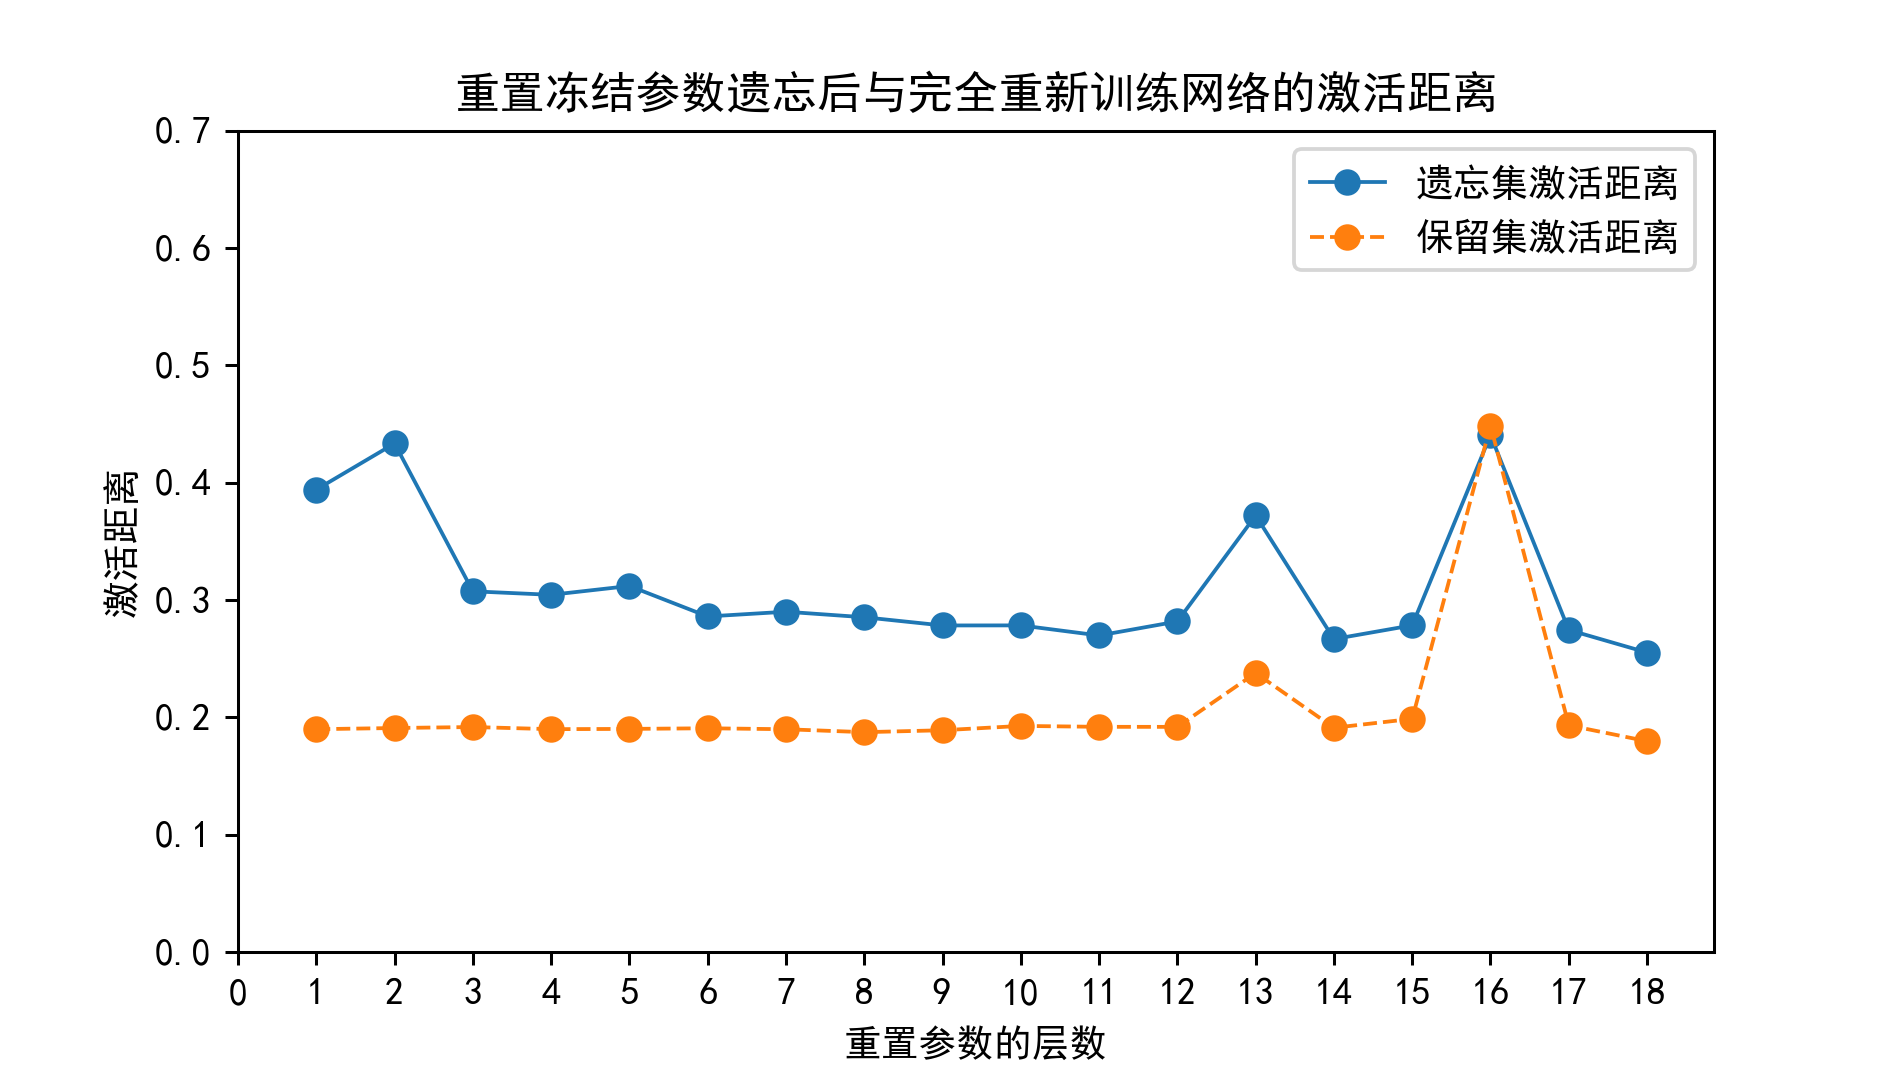
\includegraphics[width=0.9\linewidth]{chapter4_distance_1.png}
    \caption{重置冻结参数遗忘后与完全重新训练网络的激活距离}
    \label{fig:chapter4_distance_1}
\end{figure}

如图\ref{fig:chapter4_time_1}所示,图中展示了本文所讲述的重置冻结参数遗忘方法训练的网络与完全重新训练所训练的网络之间对于测试集输出之间的距离差。
这个距离差在上一节有具体讲到,是两个网络输出向量差的绝对值的第二范数值。我们用这个范数值在测试数据集上的期望来作为两个网络的激活距离。
蓝色折线代表两个网络在遗忘集上的激活距离,橙色折线代表两个网络在保留集上的激活距离。从图中可以看出,两个网络在遗忘集上的激活距离要高于在保留集上的激活距离。
我们对于两个网络激活距离的期望是越小越好,在前7层可以看到保留集的激活距离普遍稳定地保持较低数值,而对于遗忘集的激活距离前2层的数值相对较大,3、4、5层数值也略大,从第6层开始,数值变得平稳。
因此,综合图\ref{fig:chapter4_1}和图\ref{fig:chapter4_time_1}和图\ref{fig:chapter4_distance_1}的分析结果,我们选择第6层作为重置冻结参数遗忘方法对于ResNet18网络重置参数的层数。
\subsection{冻结必要性验证实验}
\begin{figure}
    \centering
    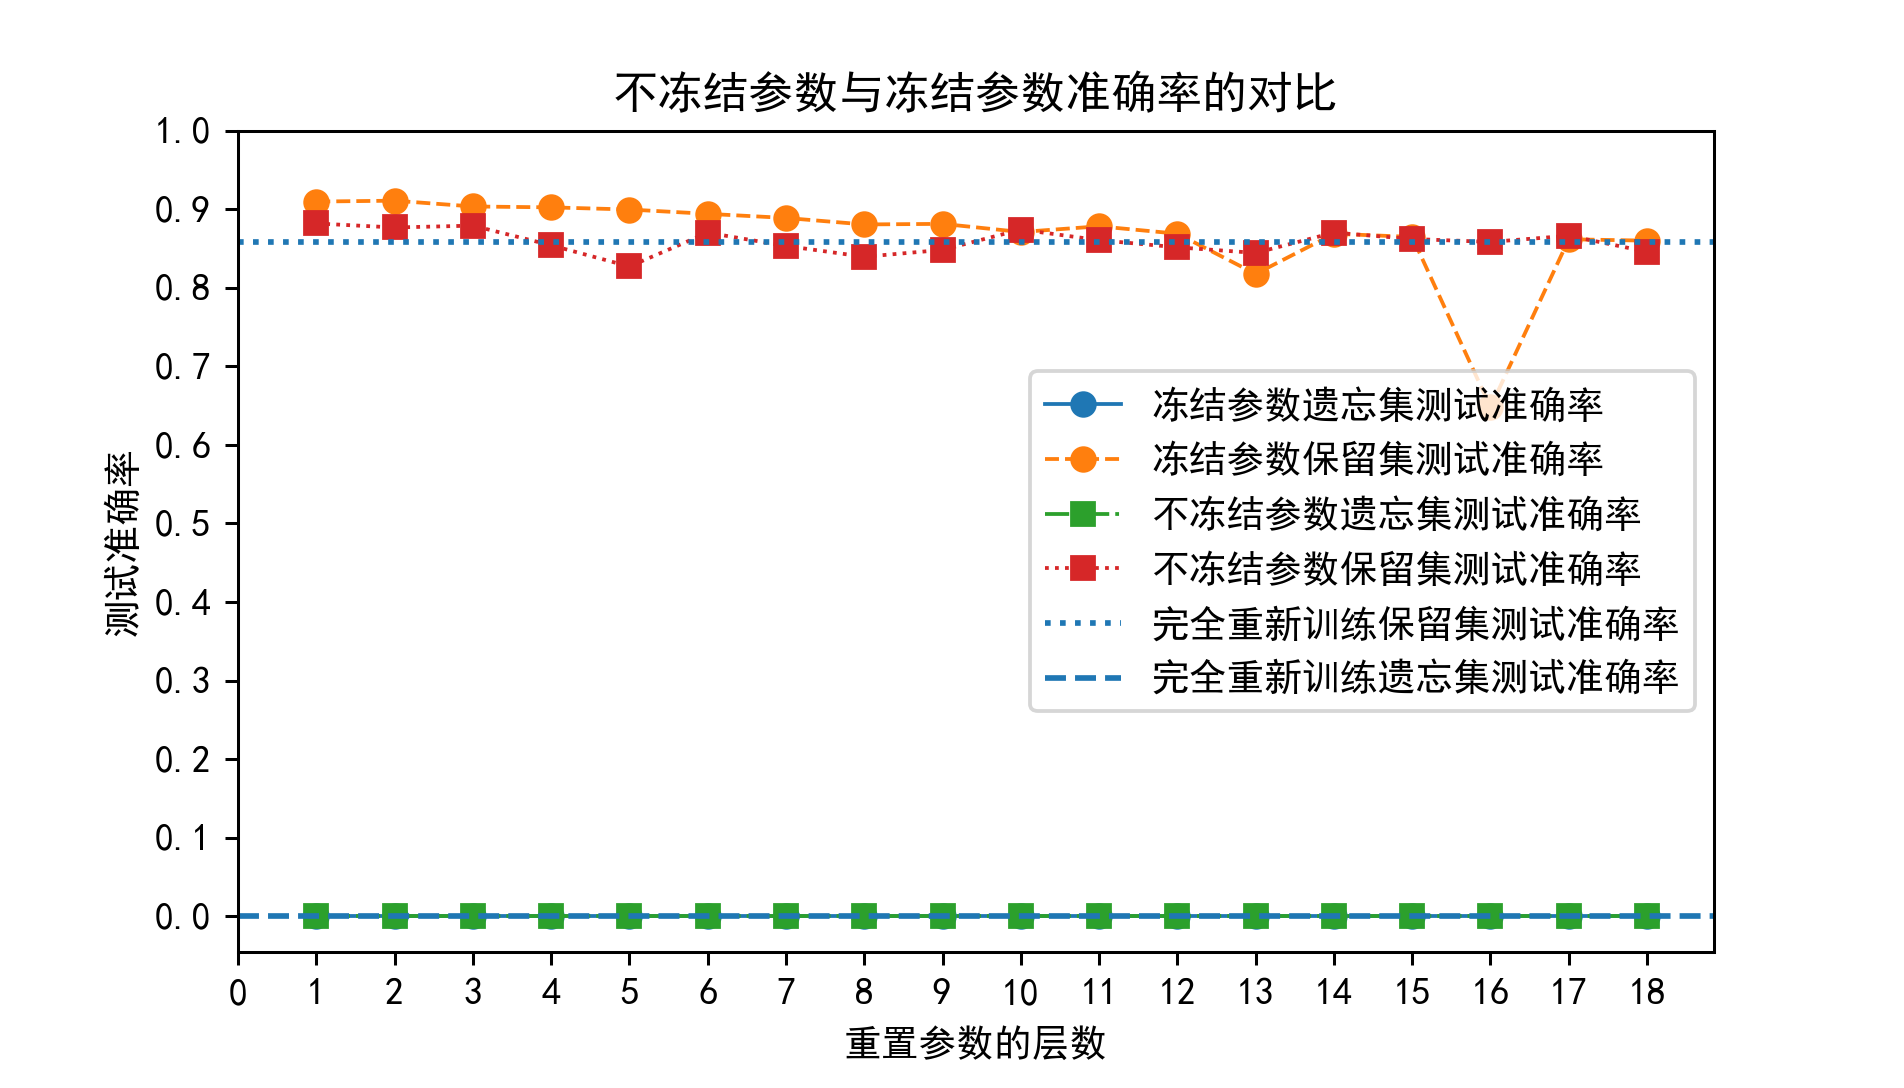
\includegraphics[width=0.9\linewidth]{chapter4_2.png}
    \caption{不冻结参数与冻结参数准确率的对比}
    \label{fig:chapter4_2}
\end{figure}

如图\ref{fig:chapter4_2}所示,图中展示了重置一定参数后冻结参数与不冻结参数训练对遗忘类别和保留类别准确率的影响。
橘黄色圆点折线代表冻结参数后使用保留训练集训练网络得到的网络在保留测试集上得到的准确率,蓝色圆点折线代表该网络的在遗忘测试集上得到的测试准确率。
红色方格折线代表不冻结参数的情况下使用保留训练集训练得到的网络在保留测试集上得到的测试准确率,绿色方格折线代表该网络在遗忘测试集上得到的测试准确率。
除此之外,图中还画了两条横线,圆点线代表完全重新训练的网络模型在保留测试集上得到的测试准确率,条状线段线代表完全重新训练的网络模型在遗忘测试集上得到的测试准确率。
这两条横线的主要作用是作为冻结参数和不冻结参数准确率的参照。通过橘黄色圆点折线和红色方格折线可以看出冻结参数与不冻结参数在保留集测试准确率上总体相差不大,但是冻结参数的方法要略好于不冻结参数方法。
在遗忘集的测试准确率上,两种方法效果相同,均为0。
\begin{figure}
    \centering
    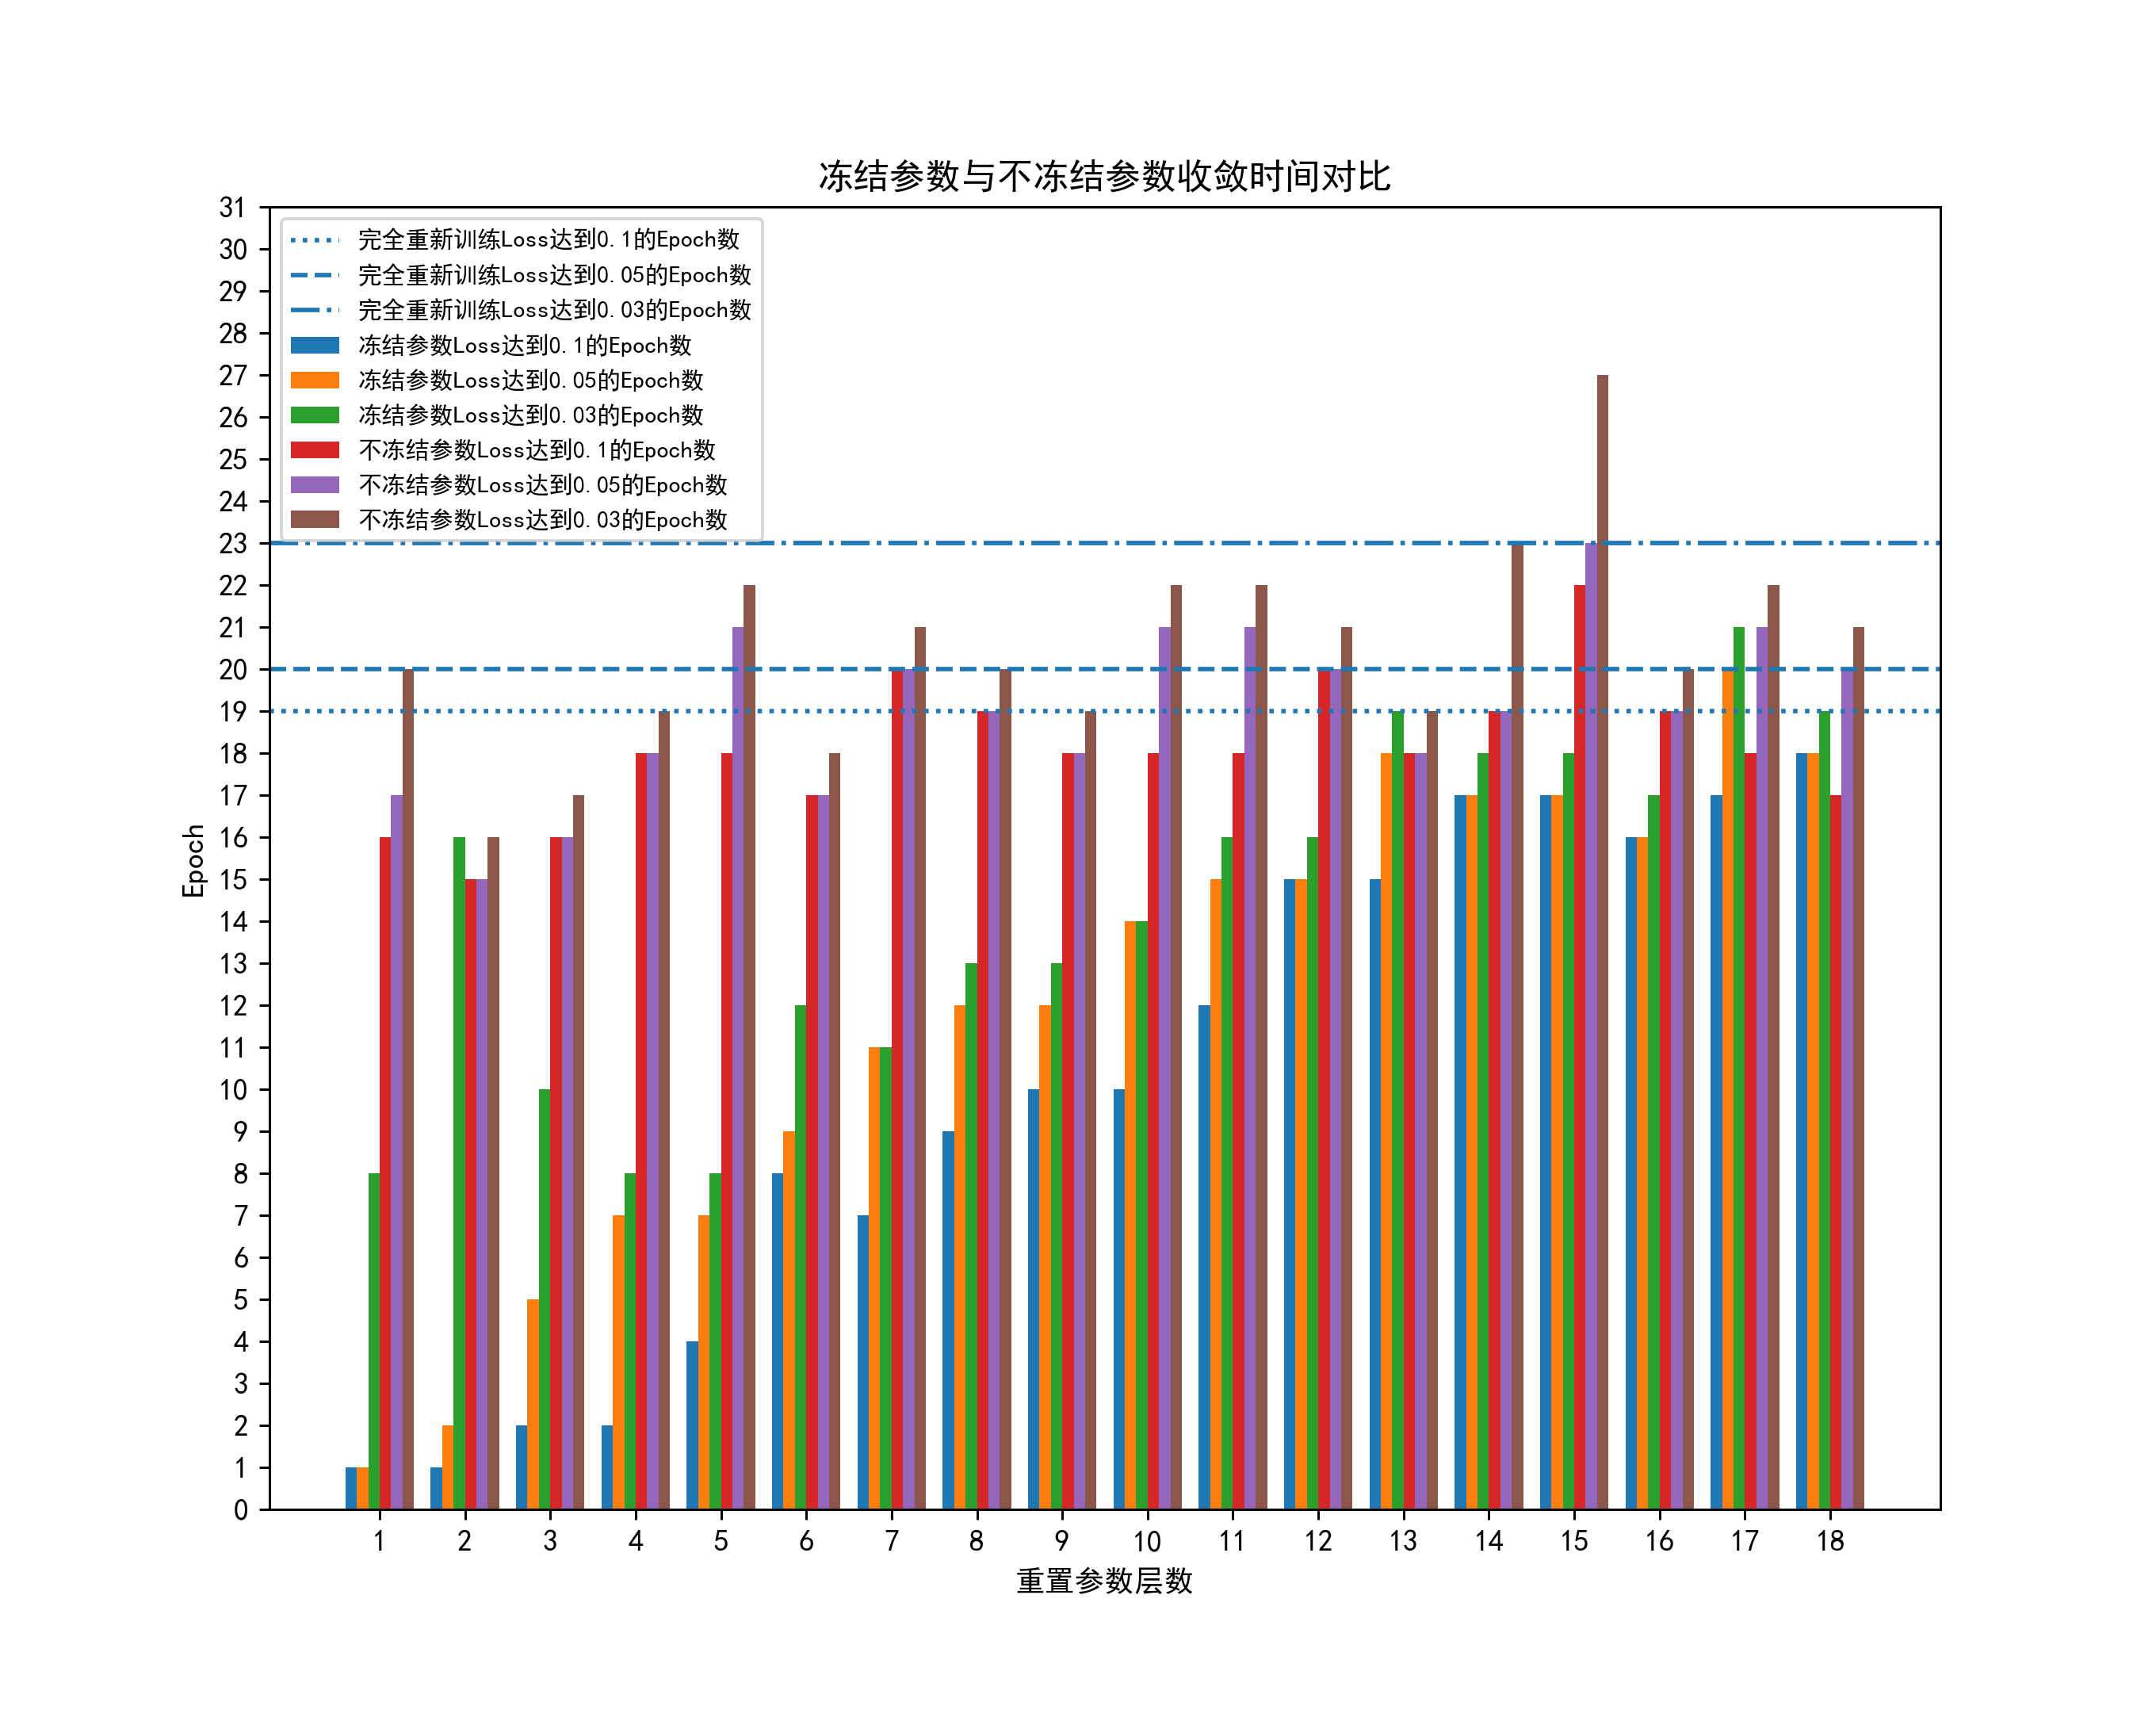
\includegraphics[width=1\linewidth]{chapter4_time_2.png}
    \caption{冻结参数与不冻结参数收敛时间对比}
    \label{fig:chapter4_time_2}
\end{figure}

如图\ref{fig:chapter4_time_2}所示,图中展示了冻结参数与不冻结参数重置参数后使用保留训练集训练网络的收敛时间。这个收敛时间同实验一的收敛时间定义相同。
蓝色、黄色和绿色柱图分别代表冻结参数情况下网络的平均损失函数值收敛到0.1、0.05和0.03时所花费的训练周期,即Epoch数。
粉色、紫色和棕色柱图分别代表非冻结参数情况下网络的平均损失函数收敛到0.1、0.05和0.03时所花费的训练周期数。
上面画出的三条横线,圆点线、条状线和点段线分别代表完全重新训练网络过程中,网络的平均损失函数值收敛至0.1、0.05和0.03时所花费的训练周期数。其主要作用是用来提供参照。
通过观察冻结参数和不冻结参数的柱状图可以发现,冻结参数后训练的收敛时间从整体上要少于不冻结参数训练网络收敛时间。这个现象也是符合分析的逻辑,冻结参数后,一部分参数不需要计算更新,而没有冻结参数的网络则需要计算所有参数的更新,从计算量上分析,不冻结参数训练网络所需要的工作量是比冻结参数要大的。
通过图\ref{fig:chapter4_2}和图\ref{fig:chapter4_time_2}的分析结果可以初步得出结论,冻结参数训练网络的方法要好于不冻结参数训练网络的方法。
\begin{figure}
    \centering
    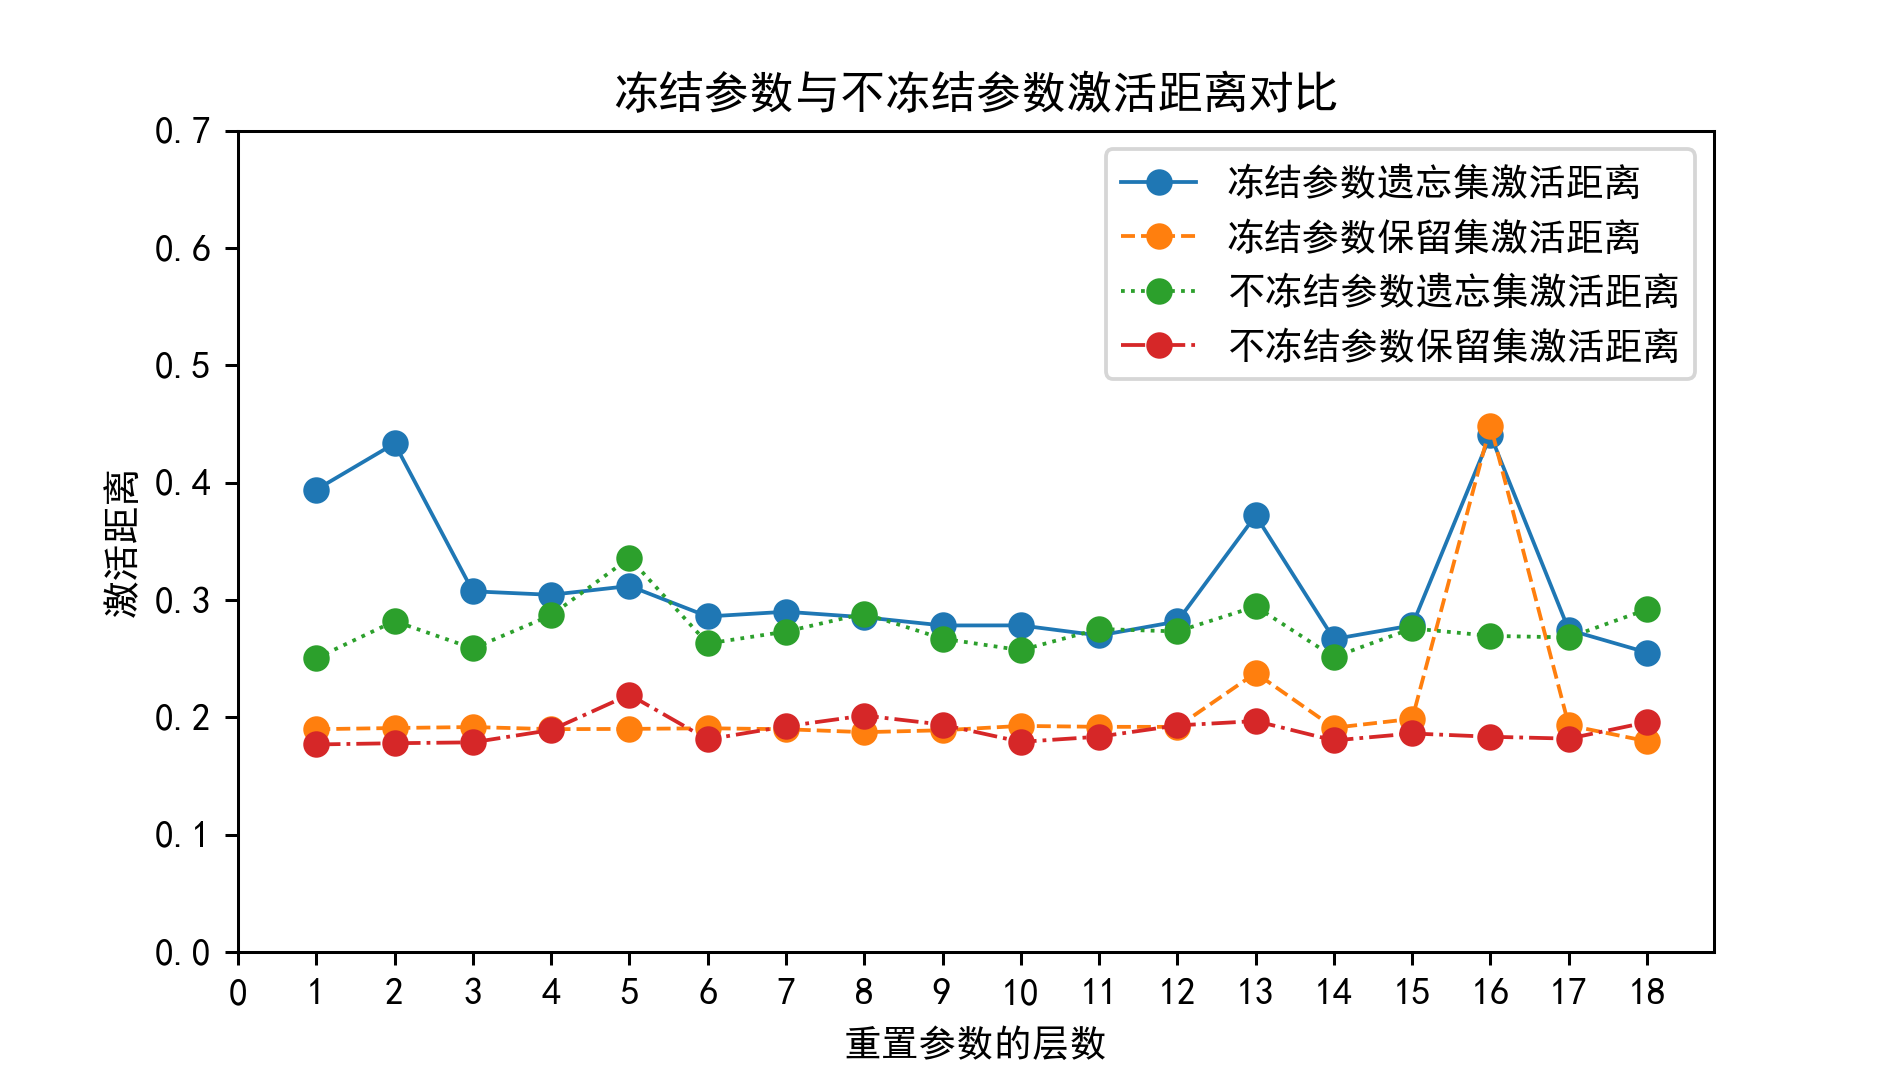
\includegraphics[width=0.9\linewidth]{chapter4_distance_2.png}
    \caption{冻结参数与没冻结参数激活距离对比}
    \label{fig:chapter4_distance_2}
\end{figure}

如图\ref{fig:chapter4_distance_2}所示,图中展示了冻结参数与不冻结参数重置参数并训练得到的两个网络在激活距离上的对比。这两个网络参照的对象均是完全重新训练生成的网络。
蓝色圆点折线和黄色圆点折线分别代表冻结参数并训练完成后,分别使用遗忘测试集和保留测试集测试网络,两个网络与重新训练的网络的输出距离。这里的距离是Softmax输出差值绝对值向量的第二范数。
同样,绿色方块折线和红色方块折线分别代表在没冻结参数情况下训练完成的网络分别用遗忘测试集和保留测试集进行测试,两个网络输出与重新训练网络输出的距离。
从图中可以看出,冻结参数的方法和没冻结参数的方法,在保留测试集上的激活距离相差无几,并且从整体水品提供商低于在遗忘测试集上产生的激活距离。
在用遗忘测试集测试的网络输出距离上,冻结参数的方法在前三层时激活距离比没冻结参数的要大,这说明只更新靠近输出的前三层冻结参数方法相比于没冻结参数的方法并不能很好的将遗忘类别很好的遗忘。

\subsection{反向冻结验证实验}
\begin{figure}
    \centering
    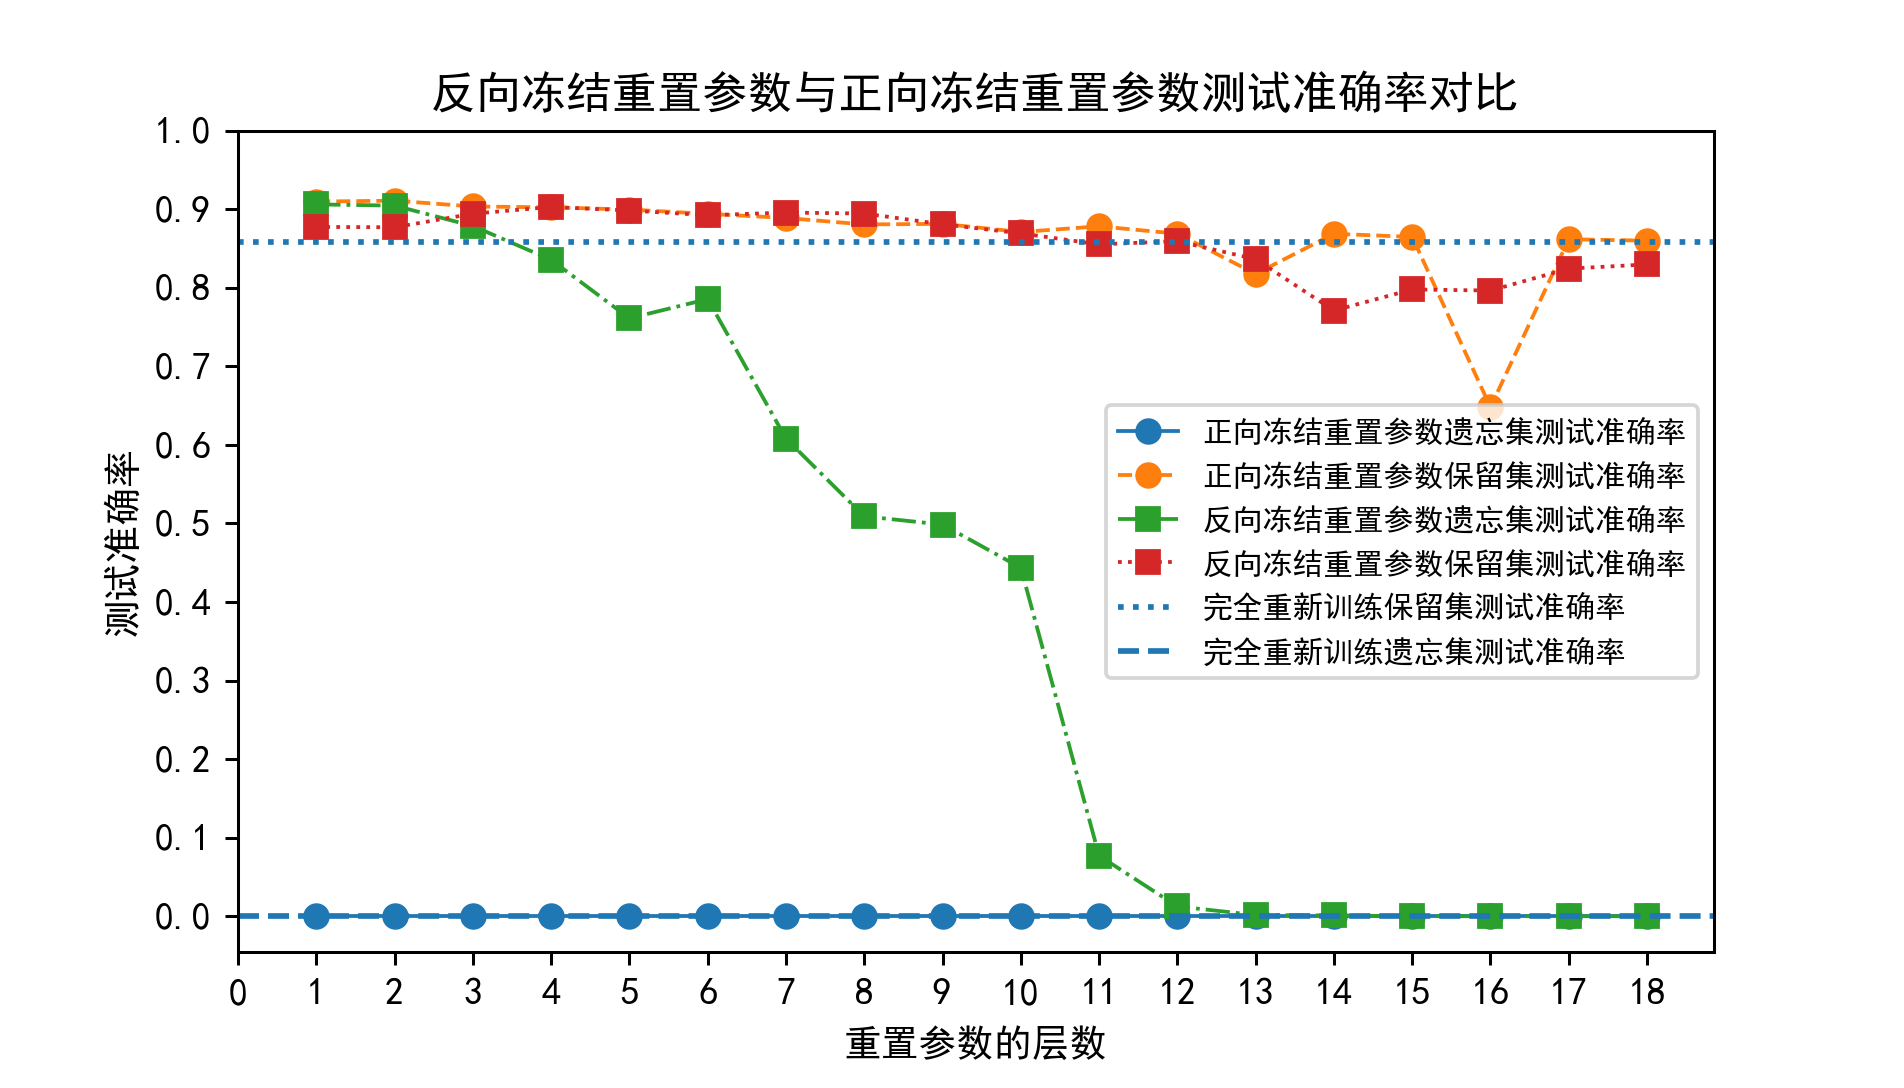
\includegraphics[width=0.9\linewidth]{chapter4_3.png}
    \caption{反向冻结重置参数与正向冻结重置参数测试准确率对比}
    \label{fig:chapter4_3}
\end{figure}

如图\ref{fig:chapter4_3}所示,图中展示了正向冻结参数与反向冻结参数训练后测试准确率的对比。
蓝色圆点圆点黄色圆点折线分别代表正向冻结参数时使用遗忘集和保留集对网络测试的准确率结果。绿色方块和红色方块折线分别代表反向冻结参数时使用遗忘集和保留集测试网络得到的准确率结果。
为了进行对比,图中还加了两条横线,圆点线代表完全重新训练网络在保留集上的测试结果,条形线代表完全重新训练网络在遗忘集上的测试准确率结果。
从图中可以看出,经过反向冻结后,保留集的测试准确率和正向冻结参数的准确率十分相近。图中,反向冻结与正向冻结最大的不同是蓝色圆点折线和绿色方块折线,他们都是在遗忘集下测试的准确率。
使用正向重置参数方法在遗忘集的测试准确率一直为0,而使用反向冻结参数方法在遗忘测试集上的准确率却是逐步在减少的。在前12层重置参数后利用保留集进行训练,遗忘集的测试准确率不为0。
这说明,重置前12层参数时并没有把遗忘类别很好地遗忘掉,有一些通过重置参数而丢失信息可以通过保留集的学习补充回去。

如果将卷积神经网络看成一半是特征提取器,另一半是分类器。这张图很好地说明了哪里是特征提取器和分类器的分界线,就是第13层,倒数第6层。
如绿色方块折线所展示的,在第13层以前,遗忘类别的分类器总能通过保留集学到的特征而产生一定的准确率。直到参数重置到了第13层,遗忘类别的分类器无法通过保留集学习到的特征而对遗忘集进行准确分类。
这就说明从第一层到第13层均有一定程度的特征提取的作用。从第13层以后,主要作用是用作分类器。我们为了彻底遗忘某个类别,我们应当是重置特征提取器的参数还是分类器的参数呢?
在这里作者认为应当更新分类器的参数。举一个例子,人类都有眼睛、鼻子和耳朵,可是影响一个人识别另一个人的因素往往不是看这个人有没有鼻子,有没有眼睛,而是眼睛和鼻子等其他器官尺寸特征。
在卷积神经网络中也是一样,低层的参数就好像在提取最基本的特征,高层的参数去提取这些基本特征之间的位置关系。所以最终影响分类的不是有没有基本特征,而是这些基本特征之间的搭配关系。
在本图中,前12层的参数被更新后,通过学习保留集,仍然能学习到遗忘集分类所用到的基本特征,所以后6层才是影响遗忘类别分类的主要参数。
\begin{figure}
    \centering
    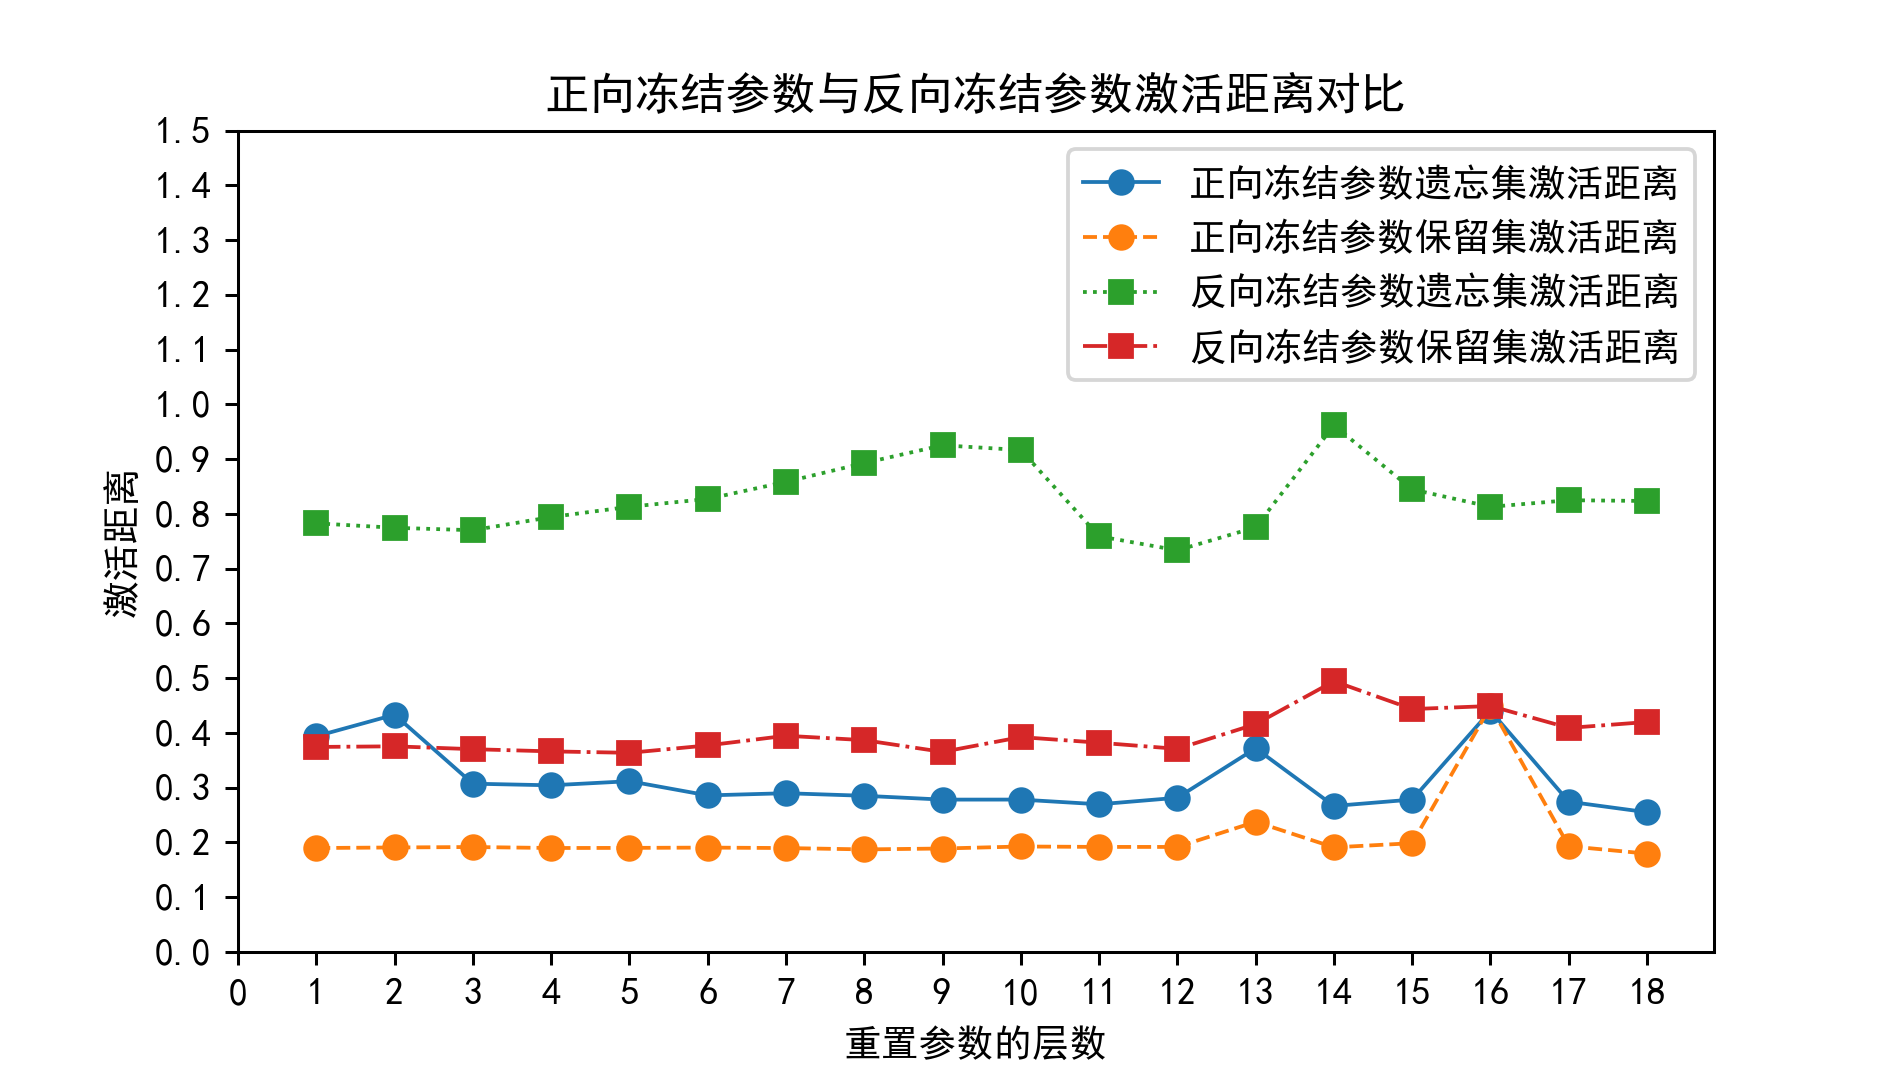
\includegraphics[width=0.9\linewidth]{chapter4_distance_3.png}
    \caption{正向冻结参数与反向冻结参数激活距离对比}
    \label{fig:chapter4_distance_3}
\end{figure}

如图\ref{fig:chapter4_distance_3}所示,图中展示了正向冻结参数与反向冻结参数的情况下,通过保留集去训练网络,再通过遗忘集和保留集分别测试网络输出距离的对比。
蓝色圆点折线和黄色圆点折线分别代表正向冻结参数的情况下训练网络,在遗忘集和给保留集上测试的网络输出距离结果。绿色方块折线和红色方块折线分别代表反向冻结参数的情况下训练网络,在遗忘集和给保留集上测试的网络输出距离结果。
从图中可以看出,蓝色圆点折线和黄色圆点折线在激活距离上面从整体上要低于绿色方块折线和红色方块折线。这说明正向冻结参数的方法要好于反向冻结参数的遗忘方法。
\subsection{遗忘可持续性验证实验}
\begin{figure}
    \centering
    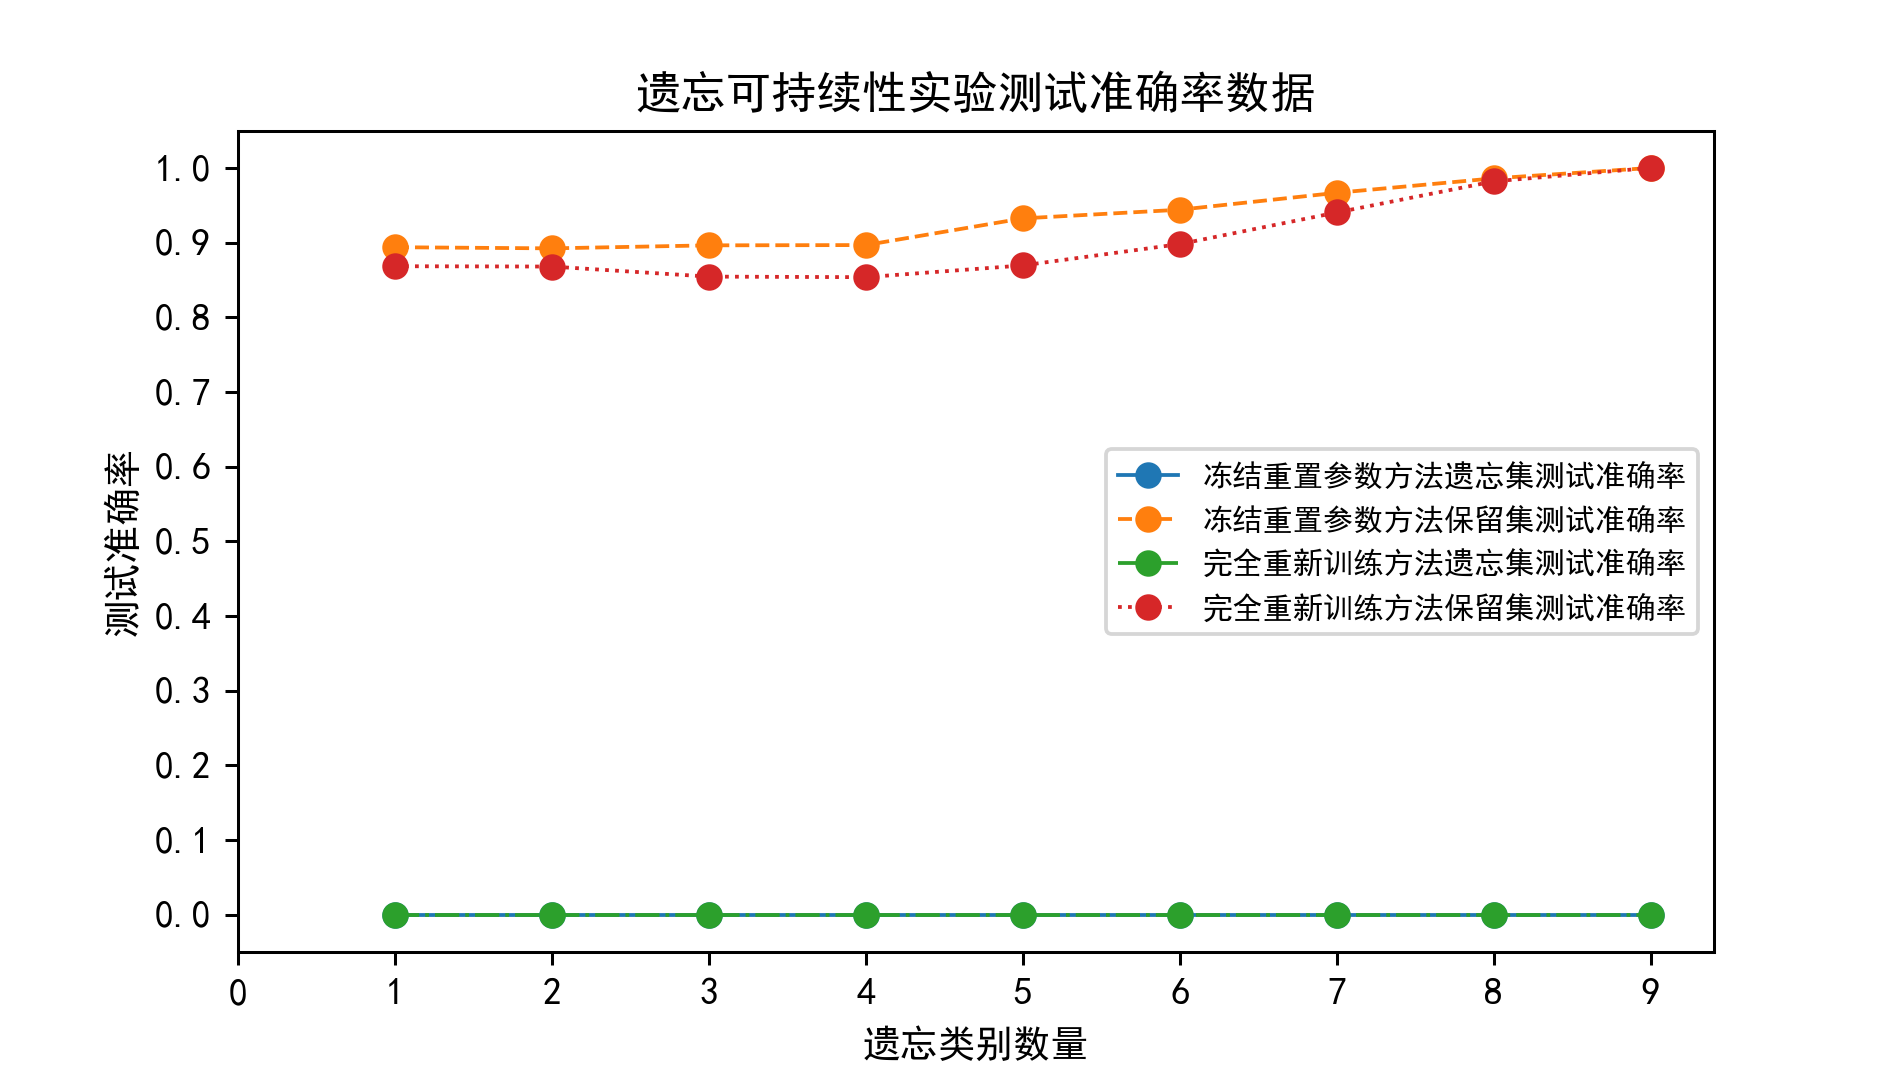
\includegraphics[width=0.9\linewidth]{chapter4_4.png}
    \caption{遗忘可持续性实验测试准确率数据}
    \label{fig:chapter4_4}
\end{figure}

如图\ref{fig:chapter4_4}所示,图中展示了遗忘可持续性实验测试准确率的结果。
图中的横轴代表遗忘类别的数量,本文使用的数据集时CIFAR-10数据集,一共又10各类别,因此遗忘类别的数量最大是9个。图中纵轴则是测试的准确率。
图中蓝色圆点折线和黄色圆点折线分别代表在冻结重置参数方法的情况下使用遗忘集和保留集测试得到的准确率结果。绿色方块折线和红色方块折线分别代表完全重新训练后,用遗忘集和保留集测试得到的测试结果。
从图中可以看出无论遗忘类别如何变化,遗忘集的测试准确率始终为0,保留集的准确率始终处于较高水平。并且和完全重新训练相比,冻结重置参数方法在保留集的测试准确率上还略高于完全重新训练的。
这说明无论遗忘掉多少类别,冻结重置参数的方法在测试准确率上是能取得很好效果的。

\begin{figure}
    \centering
    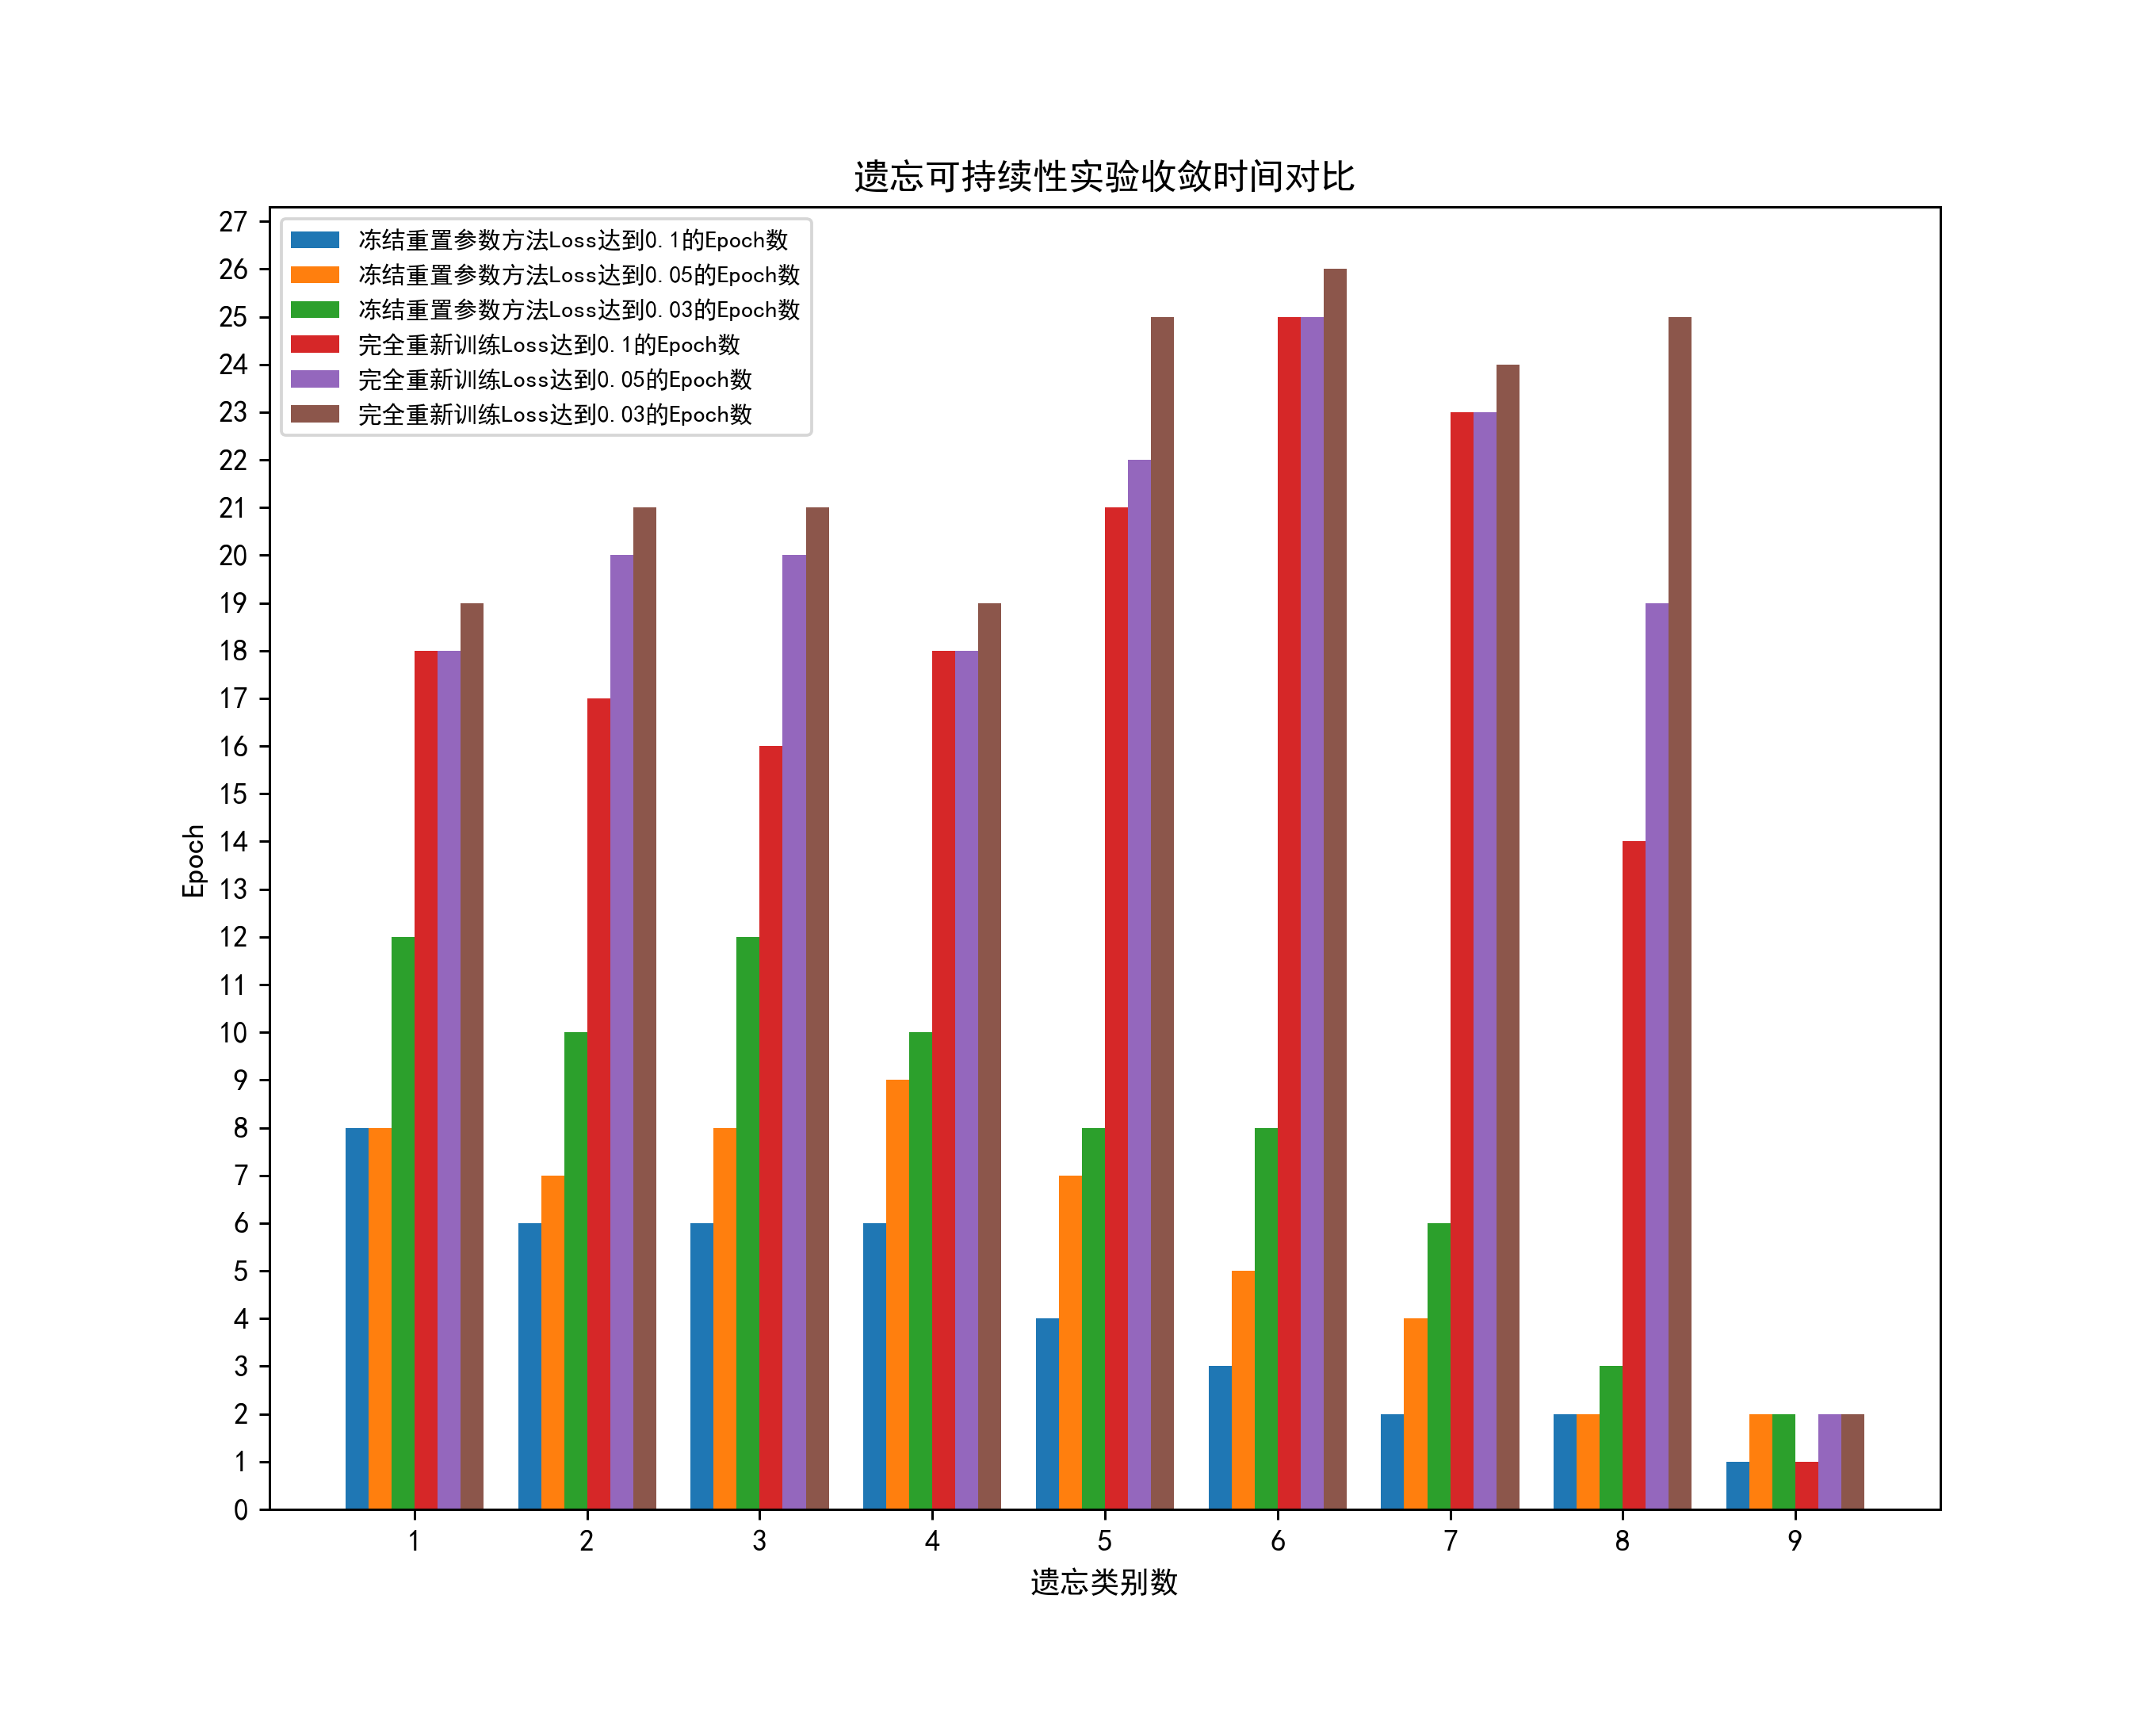
\includegraphics[width=1\linewidth]{chapter4_time_3.png}
    \caption{遗忘可持续性实验收敛时间对比}
    \label{fig:chapter4_time_3}
\end{figure}

如图\ref{fig:chapter4_time_3}所示,图中展示了遗忘可持续性实验不同遗忘类别数下收敛时间的对比情况。
图中横轴是遗忘类别数,纵轴是收敛时间,仍然使用训练过程中平均损失函数收敛至限值以下时的训练批次数来表示。
图中蓝色、黄色和绿色柱图代表冻结重置参数方法在平均损失函数收敛至0.1、0.05和0.03以下时训练批次数。红色、紫色和棕色柱图分别代表完全重新训练的情况下,平均损失函数达到0.1、0.05和0.03以下时训练批次数。
从图中可以看出,冻结重置参数方法的收敛时间从整体上要远低于完全重新训练的收敛时间。因此无论需要遗忘多少类别,冻结重置参数方法在时间上与完全重新训练相比是占有很大优势的。

\begin{figure}
    \centering
    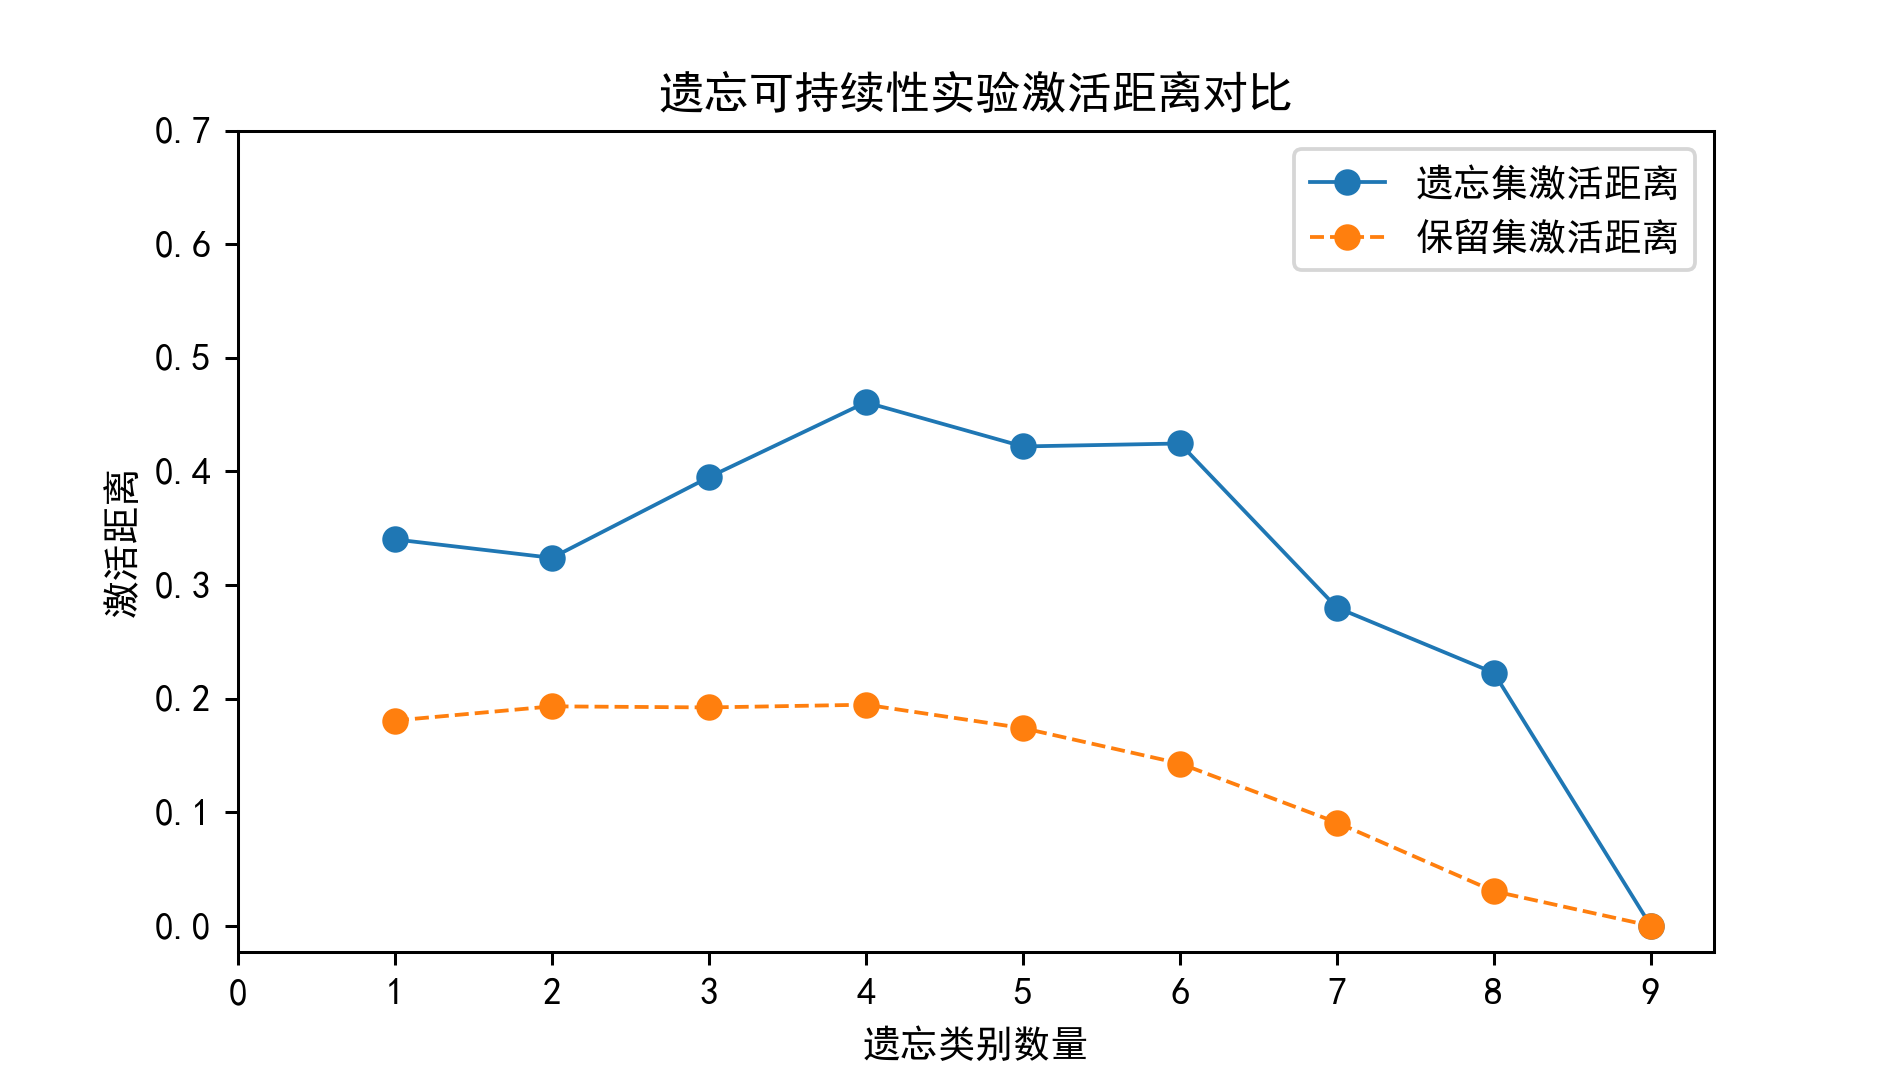
\includegraphics[width=0.9\linewidth]{chapter4_distance_4.png}
    \caption{遗忘可持续性实验激活距离对比}
    \label{fig:chapter4_distance_4}
\end{figure}

如图\ref{fig:chapter4_distance_4}所示,图中展示了遗忘可持续性实验随着遗忘类别的增加激活距离的对比情况。
图中蓝色实线代表经过冻结重置方法遗忘过后,网络在遗忘集上面与完全重新训练网络的输出距离。黄色条形线则代表两个网络在保留集上的激活距离。
从图中可以看出,从整体上,遗忘集的激活距离要高于保留集的激活距离。并且随着遗忘类别的增加,两个激活距离均有先增大后减小的趋势。不过,激活距离的最大值仍然是在0.5以下。

\section{本章小结}
本章对第三章提出的冻结重置参数的遗忘方法进行了实验验证。首先先设计了确定重置参数层次确定的实验。确定的准则通过几个指标来综合考量,一个是保留集的准确率要不能太低,遗忘集的准确率不能太高。
另一个是重新学习的时间要在可接受的范围内,并且与完全重新训练相比具有时间上面的明显竞争性。还有一个重要指标是激活距离,激活距离越近效果越好。
接下来设计了冻结和不冻结参数的对比试验,目的是验证冻结参数是有必要的。结果很好地支持了本文使用的方法,冻结参数的准确率要略高于不冻结参数的准确率,而且在重新训练时间上,相比于不冻结参数,冻结参数的方法重新学习的时间要低很多。
接下来设计了反向重置参数与正向重置参数训练的对比试验,目的是验证卷积神经网络的分层抽象特性,同时也为正向冻结参数做一个对比实验。通过反向重置参数的遗忘准确率曲线可以看出,反向重置参数并不能使得遗忘类别达到很好的遗忘效果。而正向重置参数却可以达到很好的遗忘效果。
这也就说明了正向重置参数是个很好的选择。
最后为了验证遗忘方法的遗忘可持续性,特别设计了遗忘可持续性实验。通过在准确率、激活距离和收敛时间上面的观察,可以发现无论遗忘类别的数量有多少,冻结重置参数的方法均能很好的支持。

